\documentclass[11pt,a4paper]{article}

\usepackage[T1]{fontenc}
\usepackage[utf8]{inputenc}
\usepackage{tgpagella}
\usepackage[sc]{mathpazo}
\linespread{1.04}
\usepackage{microtype}
\usepackage[a4paper,margin=2.5cm,headheight=14pt]{geometry}
\usepackage{amsmath,amssymb}
\usepackage{graphicx}
\usepackage{subcaption}
\usepackage{booktabs}
\usepackage{enumitem}
\usepackage{float}
\usepackage[section]{placeins}
\usepackage{tikz}
\usetikzlibrary{arrows.meta,positioning,calc,fit,backgrounds}
\usepackage{pgfplots}
\pgfplotsset{compat=1.17}
\usepackage{xcolor}
\usepackage{fancyhdr}
\usepackage{titlesec}
\usepackage[toc,page]{appendix}
\usepackage[numbers,sort&compress]{natbib}
\usepackage[hidelinks]{hyperref}
\usepackage[nameinlink,capitalise]{cleveref}

\graphicspath{{../figures/}}

% One palette for every diagram and chart. The four data colours are separable under the
% common forms of colour blindness and remain distinct in greyscale print.
\definecolor{ink}{HTML}{1B2A3A}
\definecolor{accent}{HTML}{0B6E8E}
\definecolor{cA}{HTML}{0072B2}
\definecolor{cB}{HTML}{D55E00}
\definecolor{cC}{HTML}{009E73}
\definecolor{cD}{HTML}{7F7F7F}
\colorlet{panel}{accent!7}
\colorlet{rule}{ink!35}

\tikzset{
  >={Stealth[length=2mm]},
  every picture/.style={line width=0.5pt, draw=ink, text=ink},
  box/.style={draw=ink, fill=panel, rounded corners=1.5pt, align=center,
              minimum height=9mm, inner sep=4pt, font=\footnotesize},
  ext/.style={box, fill=white, dashed},
  note/.style={font=\scriptsize, text=ink!80, align=center},
}
\pgfplotsset{
  report/.style={
    width=0.62\linewidth, height=0.38\linewidth,
    axis line style={draw=ink}, tick style={draw=ink},
    tick label style={font=\footnotesize}, label style={font=\footnotesize},
    legend style={font=\footnotesize, draw=none, fill=none, at={(0.5,1.04)}, anchor=south,
                  legend columns=-1, /tikz/every even column/.append style={column sep=9pt}},
    legend cell align=left,
    grid=major, grid style={draw=ink!12},
    axis lines*=left,
  }
}

% Running head: short title on the left, page number on the right.
\pagestyle{fancy}
\fancyhf{}
\fancyhead[L]{\small\textcolor{ink!80}{Trident: Design and Simulation of a Pick and Place Robot}}
\fancyhead[R]{\small\thepage}
\renewcommand{\headrulewidth}{0.3pt}
\renewcommand{\headrule}{\hbox to\headwidth{\color{rule}\leaders\hrule height \headrulewidth\hfill}}

\titleformat{\section}{\Large\bfseries\color{ink}}{\thesection}{0.6em}{}
\titleformat{\subsection}{\large\bfseries\color{ink}}{\thesubsection}{0.6em}{}
\titleformat{\subsubsection}{\normalsize\bfseries\color{ink}}{\thesubsubsection}{0.6em}{}
\titlespacing*{\paragraph}{0pt}{1.4ex plus 0.4ex}{0.8em}
\setlength{\parskip}{0pt}
\setlist{itemsep=2pt,topsep=4pt}
\captionsetup{font=small,labelfont={bf,color=ink},labelsep=period,skip=6pt}
\renewcommand{\arraystretch}{1.12}

\newcommand{\code}[1]{\texttt{#1}}
\newcommand{\unit}[1]{\ensuremath{\,\mathrm{#1}}}
\newcommand{\vect}[1]{\mathbf{#1}}

% Plan of the mission arena in metres, for use inside a tikzpicture whose x and y units are
% set to the wanted scale. Dimensions mirror src/trident_gazebo/worlds/arena.sdf.xacro.
\newcommand{\arenaplan}{%
  % floor and walls
  \fill[white] (-0.3,-0.6) rectangle (3.3,1.8);
  \draw[draw=ink, line width=1.1pt] (-0.3,-0.6) rectangle (3.3,1.8);
  \draw[draw=ink, line width=1.1pt] (0.9,-0.6) -- (0.9,0.2);
  \draw[draw=ink, line width=1.1pt] (0.9,1.0) -- (0.9,1.8);
  % entry line and start square
  \draw[draw=black, line width=0.9pt] (0,0) -- (0.15,0) arc (-90:-30:0.6) arc (150:90:0.6) -- (1.46,0.6);
  \fill[black] (1.40,0.54) rectangle (1.52,0.66);
  % pick bays: stem, crossbar, QR placard on the left wall
  \foreach \bx in {1.5,2.0,2.5} {
    \draw[draw=black, line width=0.9pt] (\bx,1.15) -- (\bx,1.45);
    \draw[draw=black, line width=0.9pt] (\bx-0.06,1.45) -- (\bx+0.06,1.45);
    \draw[draw=ink, line width=1.6pt] (\bx-0.08,1.79) -- (\bx+0.08,1.79);
  }
  % drop zones: stem, square, QR placard on the front wall
  \foreach \dy in {0.7,0.2,-0.3} {
    \draw[draw=black, line width=0.9pt] (2.575,\dy) -- (2.875,\dy);
    \fill[black!80] (2.875,\dy-0.125) rectangle (3.125,\dy+0.125);
    \draw[draw=ink, line width=1.6pt] (3.29,\dy-0.08) -- (3.29,\dy+0.08);
  }
}
% Coins in their bays, in the colour order of the default launch (red, green, blue)
\newcommand{\arenacoins}{%
  \fill[cB] (1.5,1.58) circle (0.02);
  \fill[cC] (2.0,1.58) circle (0.02);
  \fill[cA] (2.5,1.58) circle (0.02);
}
% Obstacle boxes of a preset: \arenaobstacles{1.90/0.55, 1.75/-0.15}
\newcommand{\arenaobstacles}[1]{%
  \foreach \ox/\oy in {#1} {
    \draw[draw=cB, fill=cB!35] (\ox-0.05,\oy-0.05) rectangle (\ox+0.05,\oy+0.05);
  }
}


\begin{document}

\thispagestyle{empty}
\begin{center}
  \vspace*{1.2em}
  {\small\scshape\color{accent} Technical Report\par}
  \vspace{0.9em}
  {\LARGE\bfseries\color{ink} Trident: Design and Simulation of a\par}
  \vspace{0.3em}
  {\LARGE\bfseries\color{ink} Differential-Drive Pick and Place Robot\par}
  \vspace{1.0em}
  {\color{rule}\rule{0.35\linewidth}{0.6pt}\par}
  \vspace{1.2em}
  {\large Joshua John Leo Valan Johnson\par}
  \vspace{0.3em}
  Roll No.\ 110123044\par
  National Institute of Technology Tiruchirappalli\par
  \vspace{1.0em}
  October 2026\par
  \vspace{1.6em}
  {\large\bfseries\color{ink} Abstract\par}
\end{center}
\vspace{0.2em}

\begin{quote}
\small
Trident is a small differential-drive robot that I designed and built for a competition
task: to follow a line and then to carry coloured coins, each to the bin of its colour. This
report presents the mechanical design of the robot and a simulation of it in which the
whole task is carried out autonomously.

The robot is a printed plate of $180\times150\unit{mm}$ on two N20 gearmotors and a ball
caster, designed in SolidWorks and completed with its electronics in fifteen days. Its
gripper does not lift. Two jaws with a parabolic profile, coupled by a pair of equal
involute gears and driven by one servo, cage a coin on the floor, and the robot slides it to
its destination; ridges on the jaws push the coin clear on release. A sliding condition for
a coin on a parabolic jaw is derived as the design rule for the profile. The mass properties
of the CAD model are then used to check the design. They show that the centre of mass lies
inside the support triangle but that the wheels carry only 18\,\% of the weight, which
limits the acceleration to 1.8\unit{m/s^2} at a friction coefficient of one and leaves a
tipping margin of a factor of two. The depth camera cannot see the last 0.15\unit{m} of
floor in front of the robot, and this constraint shapes the software.

The robot is modelled in Gazebo from the CAD export, with models of the depth camera, the
inertial sensor and an eight-channel infrared array. The floor markings of the mission
arena are dimensioned from the pitch of that array. Mapping, localisation and navigation
use RTAB-Map and Nav2; a line follower, docking sequences and a mission state machine were
written for the robot. The damping of the line follower is shown to be set by the distance
of the array ahead of the axle.

In twelve simulated missions with four obstacle layouts the robot delivered all 36 coins,
in 300\unit{s} per mission on average, scored by a referee on ground truth. The line was
followed within 6\unit{mm}, the pose in the map was accurate to 10\unit{mm} RMS, the robot
stopped on the pick markers within 7\unit{mm}, and coins were placed within 21\unit{mm} of
the centres of their squares.

All measurements were taken in simulation. The printed robot won the district round of the
competition and failed in the state round when its infrared array stopped working; no
measurements exist for the hardware.

\medskip
\noindent\textbf{Keywords:} mobile robot design, differential drive, caging gripper, line
following, visual SLAM, navigation, Gazebo, ROS~2.
\end{quote}

\thispagestyle{empty}
\clearpage

\tableofcontents
\clearpage

\section*{Nomenclature}
\addcontentsline{toc}{section}{Nomenclature}

\noindent\textbf{Frames and mechanics (\cref{sec:mechanical,sec:simulation})}
\begin{center}
\begin{tabular}{@{}p{0.2\linewidth}p{0.74\linewidth}@{}}
$x$, $y$ & robot frame with origin at the midpoint of the axle: $x$ forward, $y$ to the left \\
$m$, $W$ & mass and weight of the robot \\
$x_c$, $x_k$ & distance of the centre of mass and of the caster ahead of the axle \\
$N_w$, $N_k$ & static load on the two wheels together and on the caster \\
$\mu$ & coefficient of friction \\
$a_{\max}$ & largest acceleration that the wheels can transmit without slip \\
$d$, $h$ & distance of the centre of mass from an edge of the support triangle, its height above the floor \\
$r$, $b$ & wheel radius and wheel separation \\
$\omega_l$, $\omega_r$ & angular speed of the left and the right wheel \\
$v$, $\omega$ & forward speed and turn rate of the robot \\
$f$ & focal length of the parabolic jaw profile \\
$\alpha$ & angle between the jaw surface and the direction of travel \\
$\varphi$ & friction angle, $\arctan\mu$ \\
$h_c$, $x_{\min}$ & height of the camera above the floor, nearest floor point that it sees \\
\end{tabular}
\end{center}

\noindent\textbf{Line following and mission (\cref{sec:arena,sec:autonomy,sec:results})}
\begin{center}
\begin{tabular}{@{}p{0.2\linewidth}p{0.74\linewidth}@{}}
$p$ & pitch of the infrared channels \\
$V_i$, $V_{\mathrm{ref}}$ & voltage of channel $i$, voltage on a white floor \\
$d_i$ & darkness of channel $i$, from 0 on white to 1 on black \\
$e$ & offset of the line from the centre of the array, positive to the left \\
$k_p$, $k_d$ & proportional and derivative gain of the steering law \\
$\omega_{\max}$ & limit of the commanded turn rate \\
$L$ & distance of the array ahead of the axle \\
$\psi$ & heading of the robot relative to the line \\
$\omega_n$, $\zeta$ & natural frequency and damping ratio of the line-following loop \\
station pose & pose in front of a stem at which the navigation hands over to the line follower \\
marker & floor marking wider than the array: the start square, a crossbar or a drop square \\
\end{tabular}
\end{center}

\noindent\textbf{Abbreviations}
\begin{center}
\begin{tabular}{@{}p{0.2\linewidth}p{0.74\linewidth}@{}}
CAD & computer-aided design \\
EKF & extended Kalman filter \\
IMU & inertial measurement unit \\
IR & infrared \\
PD & proportional and derivative (control) \\
RMS & root mean square \\
SLAM & simultaneous localisation and mapping \\
URDF & Unified Robot Description Format \\
\end{tabular}
\end{center}
\clearpage

\section{Introduction}
\label{sec:introduction}

\subsection{Context}
Trident is a small differential-drive robot that I designed and built for a robotics task of
the WorldSkills competition. The task has two parts. The robot first follows a black line on
the floor. It then enters an area in which plastic coins, cylinders about 40\unit{mm} across
and 15\unit{mm} high, each of one colour, have to be carried to the bin of the same colour.
The first part is solved with an infrared reflectance array, the second with a camera, so the
task combines line following with vision-based navigation and a simple manipulation.

The project has passed through two versions.
\begin{enumerate}
  \item \textbf{Version 1} was a test rig: a laser-cut acrylic base with a lidar and a depth
        camera, built to learn ROS~2 and Gazebo and to see the same software run on real
        sensors (\cref{sec:evolution}).
  \item \textbf{Version 2} is the competition robot (\cref{fig:v2-intro}). Its chassis and
        gripper were designed in SolidWorks and printed, and the mechanical design and the
        electronics were completed in fifteen days before the state round of the
        competition.
\end{enumerate}
The robot won the district round. In the state round it did not complete the task, because
its infrared array stopped working. This report documents the design of Version 2 and a
simulation of it in which the whole task is carried out autonomously.

\begin{figure}[htbp]
  \centering
  \begin{subfigure}[b]{0.47\linewidth}
    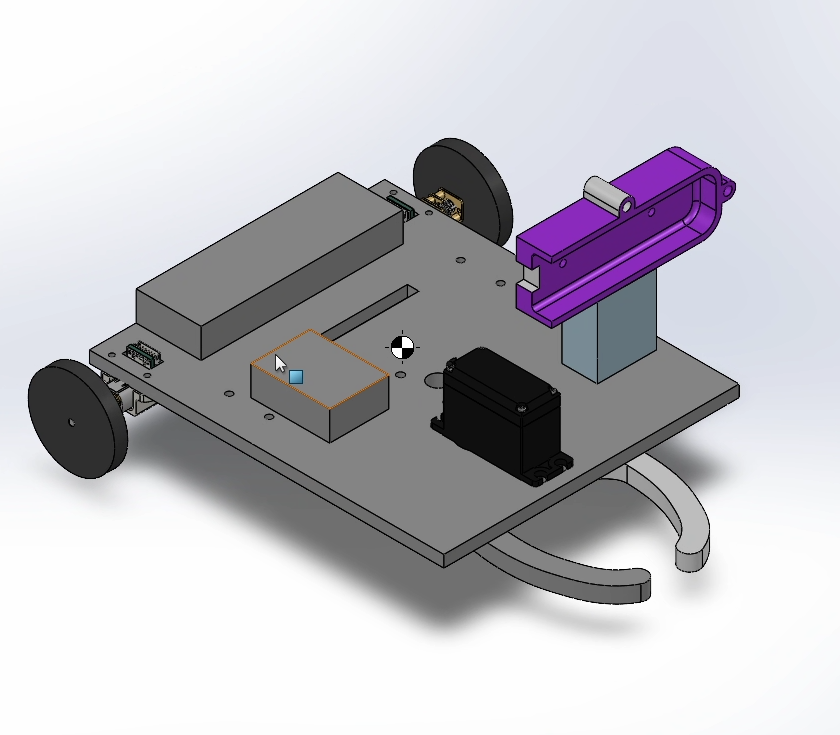
\includegraphics[width=\linewidth]{cad_iso.png}
    \caption{CAD model}
  \end{subfigure}\hfill
  \begin{subfigure}[b]{0.44\linewidth}
    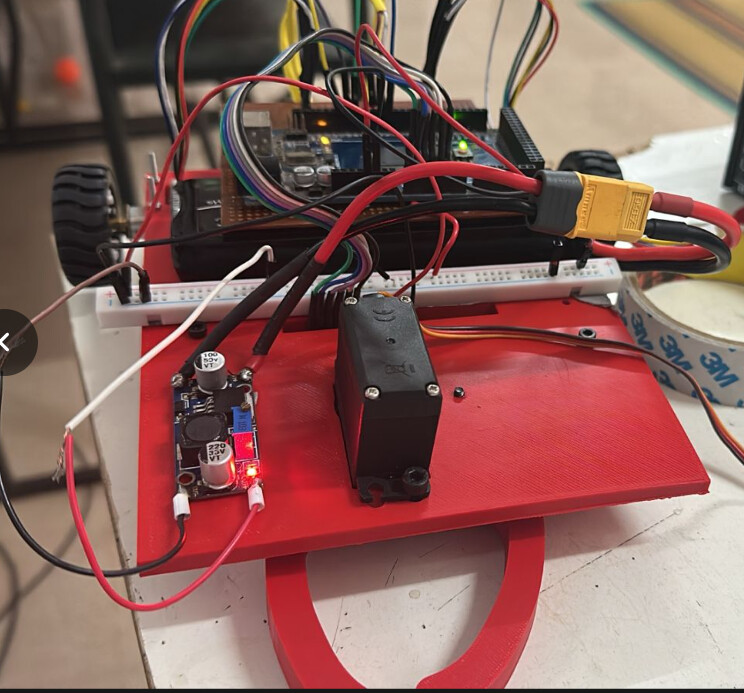
\includegraphics[width=\linewidth]{v2_hardware.jpg}
    \caption{Printed robot during wiring}
  \end{subfigure}
  \caption{Version 2 of Trident: two driven wheels at the rear, a ball caster under the plate
  and a pair of geared jaws at the front. The holder at the side of the plate carries the
  depth camera.}
  \label{fig:v2-intro}
\end{figure}

\subsection{Problem Statement and Objectives}
A robot of this size has little room for mechanism, and a robot built in two weeks has
little time for trial runs. Both facts push decisions into the design: the gripper has to
work without a lift axis and without feedback, and the software has to be tested before the
hardware is free for it. The work reported here therefore has two objectives:
\begin{enumerate}
  \item to design a chassis, a drive and a gripper that move a coin of known size reliably
        with one servo and no sensing in the jaws;
  \item to build a simulation of the robot, from the same CAD model, in which the complete
        mission can be run, scored against ground truth and repeated under varied conditions.
\end{enumerate}

\subsection{Contributions}
The contributions of this report are:
\begin{itemize}
  \item the mechanical design of the robot: its layout, drive, sensor placement and a
        gripper that cages a coin between two curved jaws and slides it along the floor
        (\cref{sec:mechanical});
  \item an analysis of that design from the mass properties of the CAD model, which gives
        the wheel loads, the traction limit and the tipping margin, and which points to
        two improvements of the layout (\cref{sec:mass});
  \item a simulation model of the robot for Gazebo, built on the CAD export, with models of
        the depth camera, the inertial sensor and the infrared array
        (\cref{sec:simulation});
  \item a mission arena whose floor markings are dimensioned from the pitch of the infrared
        array (\cref{sec:arena});
  \item an autonomy stack that combines an existing visual SLAM system and navigation
        framework with a line follower, docking sequences and a mission state machine
        written for this robot (\cref{sec:autonomy});
  \item measurements of the simulated mission over repeated runs with different coin
        orders and obstacle layouts (\cref{sec:results}).
\end{itemize}
I am the sole author of the design, the hardware and the software. Where the software uses
existing open-source packages, \cref{sec:autonomy} states which.

\subsection{Organisation}
\Cref{sec:related} places the work in context. \Cref{sec:evolution} describes the two
versions. \Cref{sec:mechanical,sec:electronics} give the mechanical design and the
electronics. \Cref{sec:simulation,sec:arena} describe the simulation model and the arena,
and \cref{sec:autonomy} the autonomy stack. \Cref{sec:results} reports the measurements,
\cref{sec:verification} the tests, and \cref{sec:discussion} the limitations.

\section{Related Work}
\label{sec:related}

\paragraph{Differential-drive platforms.} The differential drive, two independently driven
wheels on one axle with a passive third support, is the standard layout of small indoor
robots, and its kinematics and odometry are textbook material~\cite{siegwart}. Frame
conventions for such platforms in ROS are fixed by REP~105~\cite{rep105}, which this work
follows.

\paragraph{Line following.} Following a line with a row of reflectance sensors is a feedback
problem in which the lateral offset of the line under the row is the measured error. A
proportional and derivative law on that error is the common solution~\cite{astrom}. The
distance of the sensor row ahead of the axle acts as a look-ahead, as it does in pure
pursuit path tracking~\cite{purepursuit}.

\paragraph{Pushing and caging.} A gripper that surrounds an object without clamping it is
a cage: the object can move, but not escape~\cite{caging}. Moving an object by pushing it
along a support surface, and the way a pushed object slides along the pusher until the
contact is stable, were analysed by Mason~\cite{mason}. The gripper of this robot relies on
both effects in place of a lift axis.

\paragraph{Simulation.} Gazebo~\cite{gazebo} is the simulator most widely used with ROS.
This work uses its current generation, Gazebo Fortress, with ROS~2
Humble~\cite{ros2}. The robot description is exported from CAD in the URDF format.

\paragraph{Localisation and mapping.} RTAB-Map~\cite{rtabmap} is an open-source SLAM
library that builds a graph of camera views, detects when a place is seen again from visual
features, and can run in a localisation mode against a saved map. It accepts the colour and
depth streams of a stereo depth camera such as the Intel RealSense D435~\cite{realsense}.
Wheel odometry and an inertial sensor are commonly fused beforehand by an extended Kalman
filter; the \code{robot\_localization} package~\cite{robotlocalization} is the usual
implementation. The underlying theory is covered by Thrun \emph{et al.}~\cite{thrun}.

\paragraph{Navigation.} Nav2~\cite{nav2} is the navigation framework of ROS~2. It combines layered
costmaps~\cite{costmap} with a global planner, a path-tracking controller and recovery
behaviours, sequenced by a behaviour tree~\cite{behaviortrees}. This work uses its NavFn
planner, which is Dijkstra's algorithm~\cite{dijkstra} on the costmap, and the Regulated
Pure Pursuit controller~\cite{rpp}.

\paragraph{Position of this work.} None of the components above is new. The contribution
lies in the design of a robot around a specific task, and in the way the limits of that
robot (no lift axis, a camera that cannot see the floor directly in front of it) determine
how the existing components are combined with task-specific ones.

\section{Design Evolution}
\label{sec:evolution}

\subsection{Version 1: a Test Rig}
The first version was not designed for a task. It was a base cut from acrylic sheet, with a
cardboard spacer and a lidar held by bolts, two driven wheels and a caster, and an Intel
RealSense depth camera in a printed holder (\cref{fig:v1}a). I built it while learning
ROS~2 and Gazebo, in order to see the packages that I had run in simulation work with real
sensors. The same robot was modelled in Gazebo Classic, driven from a game controller and
used for lidar mapping.

On the hardware, the output of the lidar and of the depth camera was verified
(\cref{fig:v1}b). Version 1 never carried a payload and had no manipulator.

\begin{figure}[htbp]
  \centering
  \begin{subfigure}[b]{0.56\linewidth}
    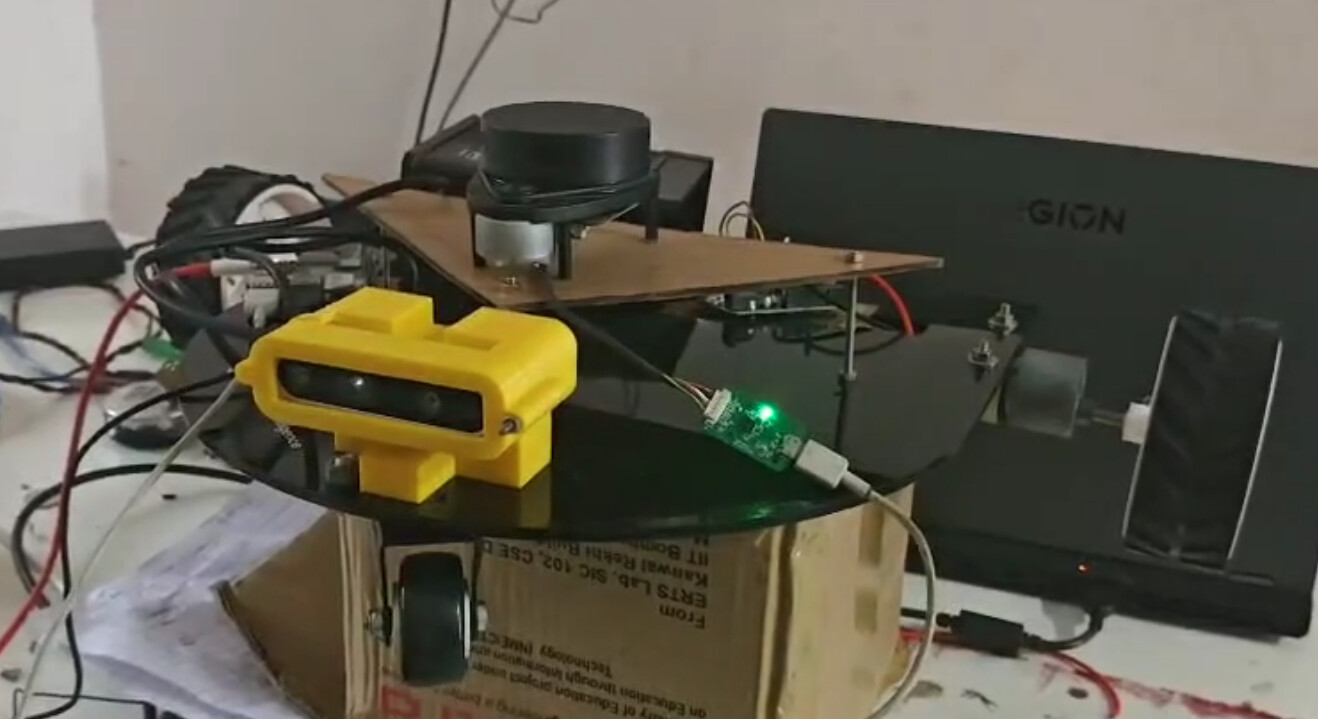
\includegraphics[width=\linewidth]{v1_rig.jpg}
    \caption{The rig with lidar and depth camera}
  \end{subfigure}\hfill
  \begin{subfigure}[b]{0.36\linewidth}
    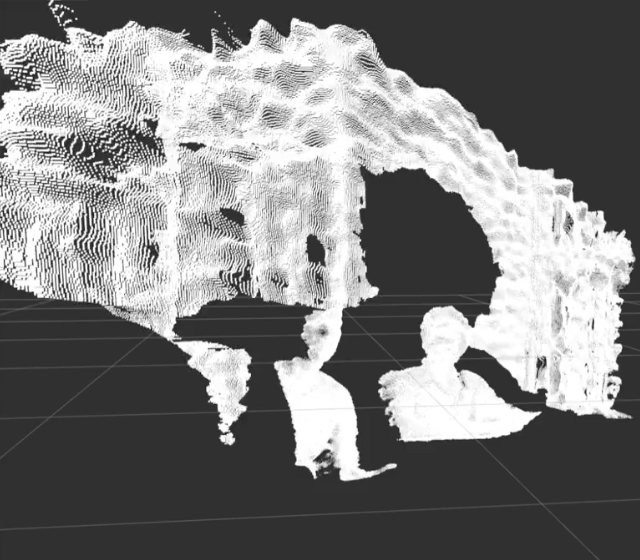
\includegraphics[width=\linewidth]{v1_depth_cloud.png}
    \caption{Depth image of the camera shown as a point cloud}
  \end{subfigure}
  \caption{Version 1, a test rig for sensors and for ROS~2.}
  \label{fig:v1}
\end{figure}

\subsection{Version 2: the Competition Robot}
Version 2 was designed for the task of \cref{sec:introduction}, and from this point the
design was deliberate. The requirements were as follows.
\begin{enumerate}
  \item The centre of mass lies inside the support triangle of the two wheels and the
        caster, so that the robot stands on all three supports.
  \item The robot is small. Motors with high torque do not fit a robot of this size, so N20
        gearmotors drive the wheels.
  \item The gripper holds a cylindrical coin about 40\unit{mm} across and 15\unit{mm} high,
        and it does so wherever the coin first touches it.
  \item The parts are printed, with tolerances that suit the bolts and nuts in use.
\end{enumerate}
The mechanical design and the electronics were completed in fifteen days. In that time the
chassis was printed in more than four iterations, each testing a different tolerance, and the
complete robot went through four iterations. The experience of Version 1 made this pace
possible.

\Cref{fig:v2-line} shows the robot on a test track for the line-following part of the task.

\begin{figure}[htbp]
  \centering
  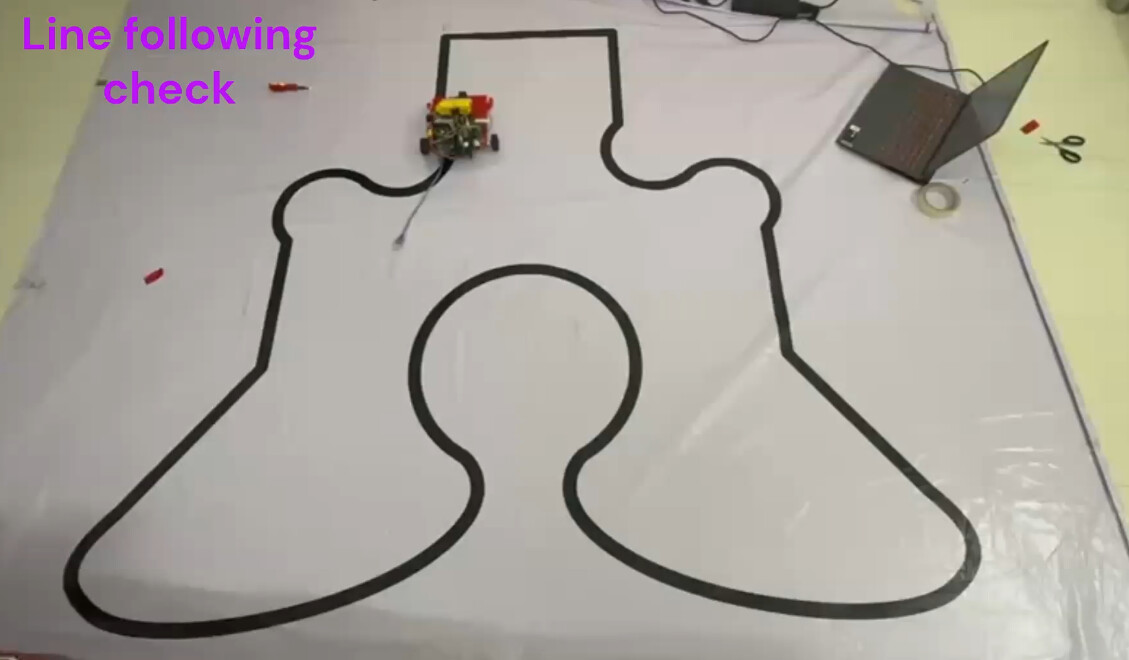
\includegraphics[width=0.62\linewidth]{v2_line_following.jpg}
  \caption{Version 2 following a line on a test track.}
  \label{fig:v2-line}
\end{figure}

\subsection{From the Hardware to the Simulation}
The simulation reported here was written after the competition, from the CAD model of
Version 2. It serves two purposes. It is a place in which the whole mission can be developed
and repeated without the hardware, and it is a check on the design: quantities that were
judged by eye during the fifteen days, such as the load that the wheels carry, can be
read from the model and their consequences calculated. \Cref{sec:mass} does this.

\section{Mechanical Design}
\label{sec:mechanical}

The robot was modelled in SolidWorks. This section gives the layout, the mass properties and
what follows from them, the drive, the gripper and the placement of the sensors. Dimensions
and masses are those of the CAD model as exported for the simulation
(\code{trident.urdf.xacro}); none of them was measured on the printed robot.

\subsection{Layout}
\label{sec:layout}
The chassis is a single printed plate of $180\times150\times6\unit{mm}$
(\cref{fig:cad-views}). Two N20 gearmotors are fixed under its rear edge and drive two
wheels of 22\unit{mm} radius, 195.5\unit{mm} apart. A ball caster under the plate, 85\unit{mm}
ahead of the axle, is the third support. The servo of the gripper stands on the plate near
the front edge, with its shaft pointing down through the plate, and the two jaws turn in a
horizontal plane below the plate and reach forward of it. The infrared array hangs under the
plate between the axle and the caster, and the depth camera sits in a holder on a post at the
left side of the plate. The battery and the control electronics occupy the rear of the plate
above the axle.

\begin{figure}[htbp]
  \centering
  \begin{subfigure}[b]{0.30\linewidth}
    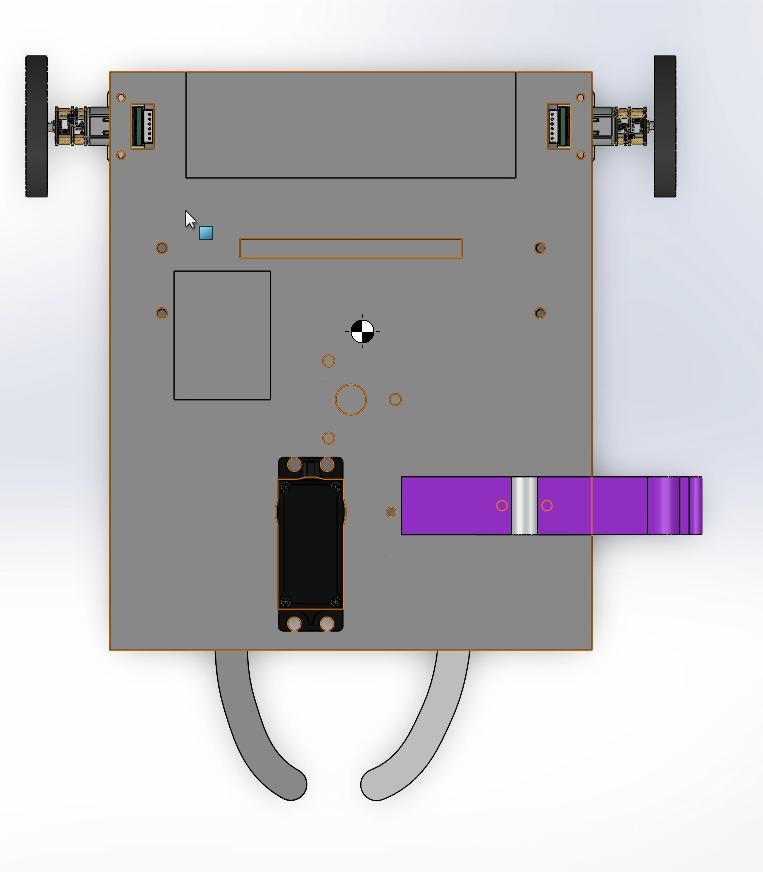
\includegraphics[width=\linewidth]{cad_top.png}
    \caption{Top}
  \end{subfigure}\hfill
  \begin{subfigure}[b]{0.30\linewidth}
    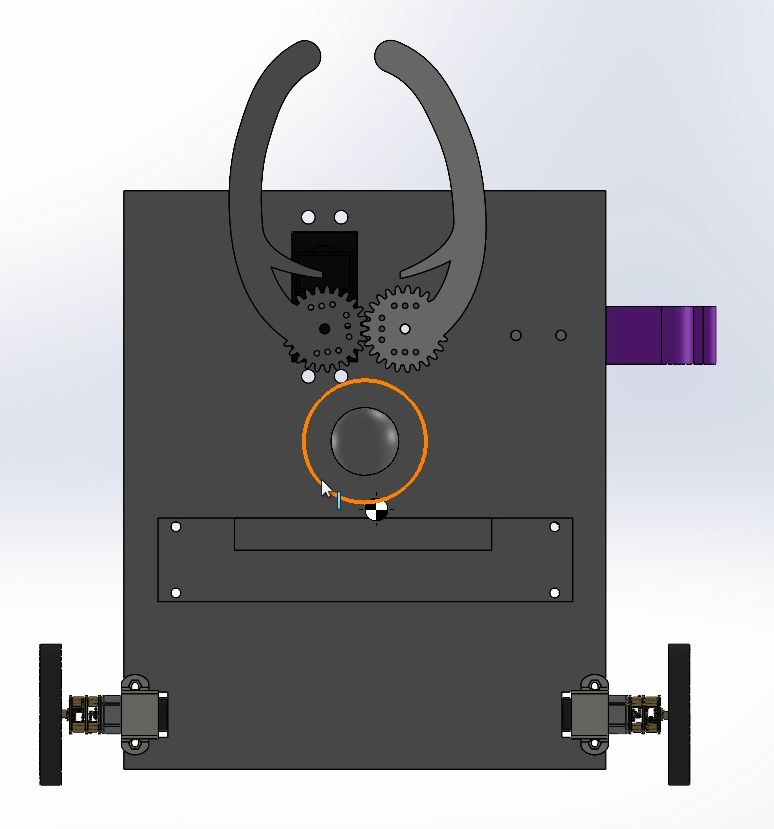
\includegraphics[width=\linewidth]{cad_bottom.png}
    \caption{Bottom}
  \end{subfigure}\hfill
  \begin{subfigure}[b]{0.36\linewidth}
    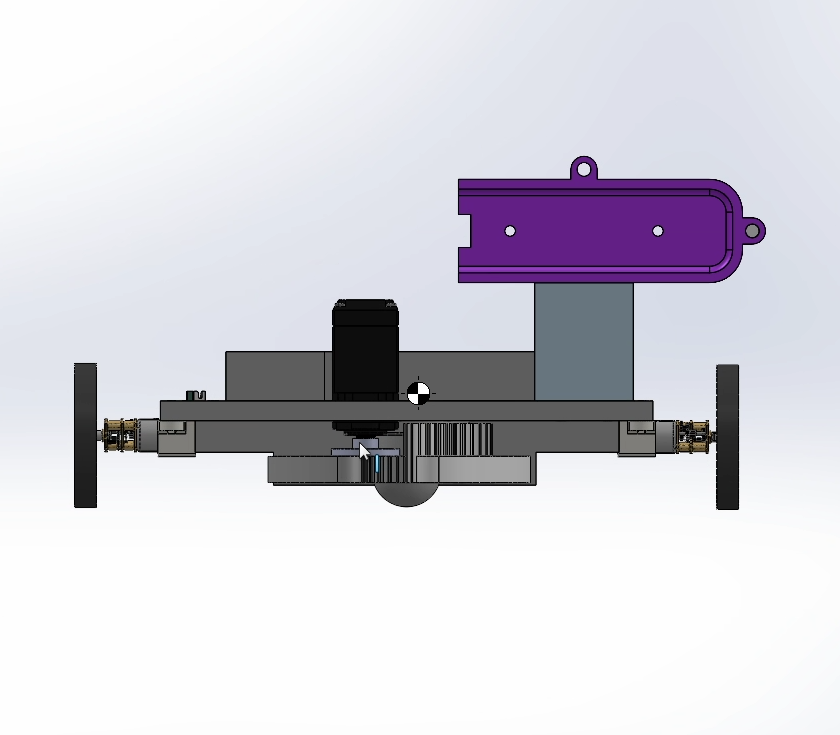
\includegraphics[width=\linewidth]{cad_front.png}
    \caption{Front}
  \end{subfigure}
  \caption{CAD model of Version 2. The black and white disc marks the centre of mass
  calculated by the CAD program. In the bottom view the caster is the dome at the centre and
  the two gears of the gripper are in front of it.}
  \label{fig:cad-views}
\end{figure}

\Cref{tab:dimensions} lists the principal dimensions.

\begin{table}[htbp]
  \centering
  \caption{Principal dimensions of the robot, from the CAD model.}
  \label{tab:dimensions}
  \begin{tabular}{@{}ll@{}}
    \toprule
    Quantity & Value \\
    \midrule
    Chassis plate & $180\times150\times6\unit{mm}$ \\
    Wheel radius, wheel separation & 22\unit{mm}, 195.5\unit{mm} \\
    Caster ahead of the axle & 85.0\unit{mm} \\
    Jaw pivots: ahead of the axle, apart & 120.0\unit{mm}, 25.0\unit{mm} \\
    Reach of a jaw from its pivot & 90\unit{mm} \\
    Infrared array: ahead of the axle, above the floor & 48\unit{mm}, 7.4\unit{mm} \\
    Infrared channels, pitch & 8, 15\unit{mm} \\
    Camera: above the floor, left of the centre line & 85\unit{mm}, 54\unit{mm} \\
    Total mass of the model & 0.64\unit{kg} \\
    \bottomrule
  \end{tabular}
\end{table}

\subsection{Mass Properties and Their Consequences}
\label{sec:mass}
The first requirement of \cref{sec:evolution} concerns the centre of mass. The CAD export
gives a mass and a centre of mass for every part, so the requirement can be checked
(\cref{tab:mass}). The origin is the midpoint of the axle, $x$ points forward and $y$ to
the left.

\begin{table}[htbp]
  \centering
  \caption{Mass budget of the model. The chassis assembly is the plate with the motors, the
  servo and the blocks that stand for battery and electronics in the CAD model.}
  \label{tab:mass}
  \begin{tabular}{@{}lrrr@{}}
    \toprule
    Part & Mass [g] & $x$ [mm] & $y$ [mm] \\
    \midrule
    Chassis assembly & 425.6 & 50.2 & $-5.5$ \\
    Depth camera (D435) & 72.0 & 129.5 & 54.3 \\
    Camera holder & 58.8 & 116.2 & 58.1 \\
    Jaws (two) & 34.8 & 146.4 & 0.3 \\
    Wheels (two) & 20.2 & 0.0 & 0.0 \\
    Infrared array & 20.0 & 49.7 & 0.0 \\
    Caster & 8.9 & 85.0 & 0.0 \\
    \midrule
    Robot & 640.3 & 69.3 & 7.8 \\
    \bottomrule
  \end{tabular}
\end{table}

\paragraph{Wheel loads.} The centre of mass lies 69.3\unit{mm} ahead of the axle and the
caster 85.0\unit{mm}. With $W=mg=6.28\unit{N}$, the caster at $x_k$ and the centre of mass
at $x_c$, the static loads are
\begin{equation}
  N_k = W\,\frac{x_c}{x_k} = 5.12\unit{N}, \qquad
  N_w = W\Bigl(1-\frac{x_c}{x_k}\Bigr) = 1.16\unit{N},
  \label{eq:loads}
\end{equation}
where $N_w$ is the sum over both wheels. The centre of mass is inside the support triangle,
as required. It lies closer to the caster than to the axle: in the model the wheels carry 18\,\% of the
weight and the caster 82\,\%. The camera with its holder, 131\unit{g} at the front of the
plate, and the jaws are responsible. The CAD views of \cref{fig:cad-views} agree with this:
the centre-of-mass mark lies next to the caster.

\paragraph{Traction limit.} The wheel load bounds the force that the wheels can transmit.
With a coefficient of friction $\mu$ between tyre and floor,
\begin{equation}
  a_{\max} = \frac{\mu N_w}{m} = \mu g\Bigl(1-\frac{x_c}{x_k}\Bigr) = 1.8\,\mu\unit{m/s^2},
  \label{eq:traction}
\end{equation}
so that even with $\mu=1$ the robot cannot accelerate or brake at more than
1.8\unit{m/s^2} without slip. This limit is visible in the simulation. With no limit on the
deceleration, the wheels of the simulated robot stopped at once on a stop command and the
robot skidded and turned; the drive is now limited to 1.0\unit{m/s^2}
(\cref{sec:sim-drive}). The force needed to slide a coin, by contrast, is small: a coin of
23\unit{g} with a friction coefficient of 0.35 resists with 0.08\unit{N}.

\paragraph{Tipping margin.} On three supports the robot tips about an edge of the support
triangle (\cref{fig:triangle}). The triangle is narrow at the caster, and the centre of mass
is both far forward and, because of the camera, 7.8\unit{mm} to the left. Its distance to
the left edge of the triangle is $d=6.7\unit{mm}$ and to the right edge 16.9\unit{mm}. With
the centre of mass at a height $h=42\unit{mm}$ above the floor, a horizontal acceleration
$a$ directed across the left edge tips the robot when $a>g\,d/h=1.6\unit{m/s^2}$. A braking
deceleration acts along $x$, at an angle to that edge, and tips the robot above
2.1\unit{m/s^2}. Both values are above the 1.0\unit{m/s^2} that the drive is allowed, but
the margin is a factor of two and not more.

\begin{figure}[htbp]
  \centering
  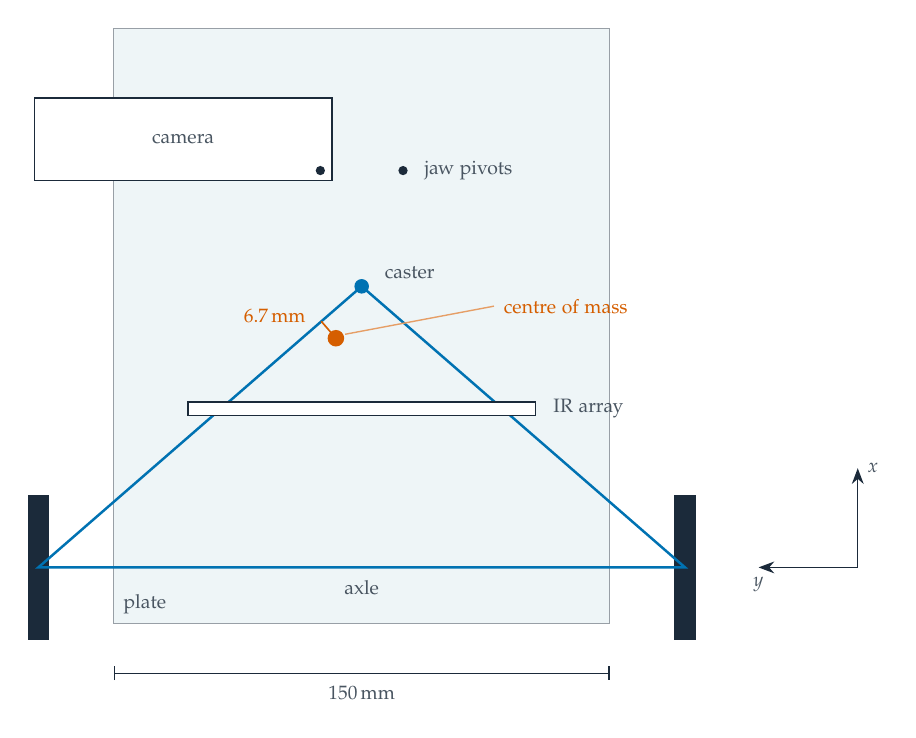
\begin{tikzpicture}[scale=0.42]
    % units: 10 mm. x forward is drawn upward, y left is drawn to the left.
    \draw[draw=ink!45, fill=panel] (-7.5,-1.7) rectangle (7.5,16.3);
    \node[note, anchor=south west] at (-7.5,-1.7) {plate};
    % wheels
    \fill[ink] (-10.1,-2.2) rectangle (-9.45,2.2);
    \fill[ink] (9.45,-2.2) rectangle (10.1,2.2);
    % support triangle
    \draw[cA, line width=0.9pt] (-9.777,0) -- (9.777,0) -- (0,8.5) -- cycle;
    \fill[cA] (0,8.5) circle (0.22);
    \node[note, anchor=west] at (0.4,8.9) {caster};
    \node[note, anchor=north] at (0,-0.1) {axle};
    % centre of mass
    \fill[cB] (-0.78,6.93) circle (0.25);
    \draw[draw=cB!60] (-0.5,7.05) -- (4.0,7.9);
    \node[note, anchor=west, text=cB] at (4.0,7.9) {centre of mass};
    \draw[cB, line width=0.6pt] (-0.78,6.93) -- (-1.22,7.44);
    \node[note, anchor=east, text=cB] at (-1.4,7.6) {6.7\,mm};
    % camera and gripper pivots
    \draw[draw=ink, fill=white] (-9.9,11.7) rectangle (-0.9,14.2);
    \node[note] at (-5.4,12.95) {camera};
    \fill[ink] (-1.25,12.0) circle (0.14);
    \fill[ink] (1.25,12.0) circle (0.14);
    \node[note, anchor=west] at (1.6,12.0) {jaw pivots};
    % IR array
    \draw[draw=ink, fill=white] (-5.25,4.6) rectangle (5.25,5.0);
    \node[note, anchor=west] at (5.5,4.8) {IR array};
    % axes
    \draw[->] (15,0) -- (15,3) node[note, right] {$x$};
    \draw[->] (15,0) -- (12,0) node[note, below] {$y$};
    % scale
    \draw[|-|] (-7.5,-3.2) -- (7.5,-3.2);
    \node[note, below] at (0,-3.3) {150\,mm};
  \end{tikzpicture}
  \caption{Support triangle of the two wheels and the caster, seen from above, to scale.
  The centre of mass of the model lies inside it, 16\unit{mm} behind the caster and
  6.7\unit{mm} from the left edge.}
  \label{fig:triangle}
\end{figure}

\paragraph{What this means for the design.} The layout meets its requirement, and the
analysis shows where it can be improved. Two changes would raise the wheel load and the
tipping margin: moving the caster forward, towards the gripper pivots, which widens the
triangle around the centre of mass and transfers load to the wheels; and mounting the
camera on the centre line, which removes the lateral offset.
Two reservations apply. The masses are CAD values, and the blocks that stand for the
battery and the electronics need not carry their true mass, so the real centre of mass may
lie further back than \cref{tab:mass} says. And the printed robot has not been weighed
on its three supports, which would settle the question in a few minutes.

\subsection{Drive}
\label{sec:drive}
The robot is a differential drive. With wheel radius $r$, wheel separation $b$ and wheel
speeds $\omega_l$, $\omega_r$, the forward speed and the turn rate are
\begin{equation}
  v = \frac{r}{2}(\omega_r+\omega_l), \qquad \omega = \frac{r}{b}(\omega_r-\omega_l).
  \label{eq:diffdrive}
\end{equation}
N20 gearmotors were chosen because motors of higher torque do not fit under a plate of this
size. The simulation assumes a variant with a no-load speed of 300\unit{rpm} at
6\unit{V} and a stall torque of 0.05\unit{N\,m} at the wheel; both are placeholders in the
model and have to be replaced by the data of the motors fitted. On these values the robot
has a top speed of $r\,\omega=0.69\unit{m/s}$, and the mission uses at most
0.20\unit{m/s}, less than a third of it. The two motors together can push with
4.5\unit{N} at stall, about four times the 1.16\unit{N} that the wheels can transmit by
\cref{eq:loads}. The drive is therefore limited by traction and not by torque, which is a
further reason to move load onto the wheels.

The wheels are narrow, and the caster is a ball that slides. In the simulation the caster
is given no friction, so that turning on the spot is resisted only by the wheels.

\subsection{Gripper}
\label{sec:gripper}
\subsubsection{Caging in Place of Lifting}
The robot is light, and a coin of unknown mass held out in front of the caster could tip it
forward. The gripper therefore does not lift. Two jaws close around the coin on the floor,
and the robot slides the coin to its destination. The jaws need not clamp: it is enough that
the coin cannot leave the space between them. This removes the lift axis and its actuator,
and it removes the need to know the mass of the coin. It also sets a condition on the floor,
which must be flat enough for a coin 15\unit{mm} high to slide; on the printed robot the
grip held on mildly uneven ground.

The jaws are 8\unit{mm} thick and their mid-plane is 12\unit{mm} above the floor, so they
meet the upper half of the rim of a coin.

\subsubsection{Jaw Profile}
The jaws were drawn with a parabolic profile (\cref{fig:gripper}a). The intent is that a
coin which meets a jaw anywhere along its length is led inward, to the region around the
focus of the parabola, where the closed jaws hold it. The robot therefore does not have to
arrive exactly in line with the coin.

\begin{figure}[htbp]
  \centering
  \begin{subfigure}[b]{0.32\linewidth}
    \centering
    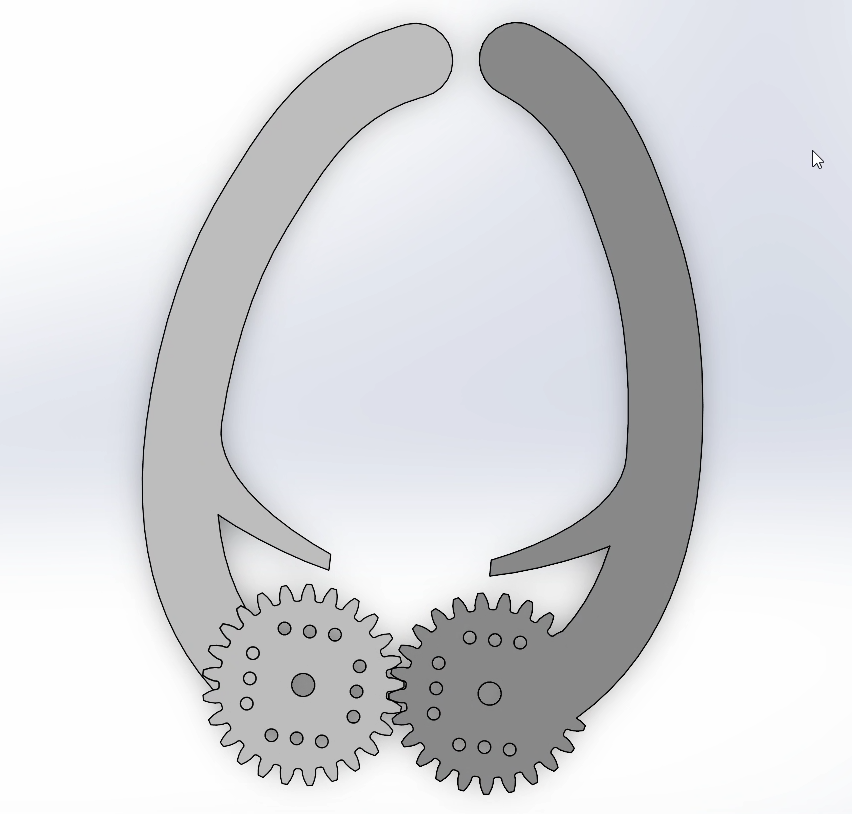
\includegraphics[width=\linewidth]{gripper_cad.png}
    \caption{Jaws and gear pair in CAD}
  \end{subfigure}\hfill
  \begin{subfigure}[b]{0.64\linewidth}
    \centering
    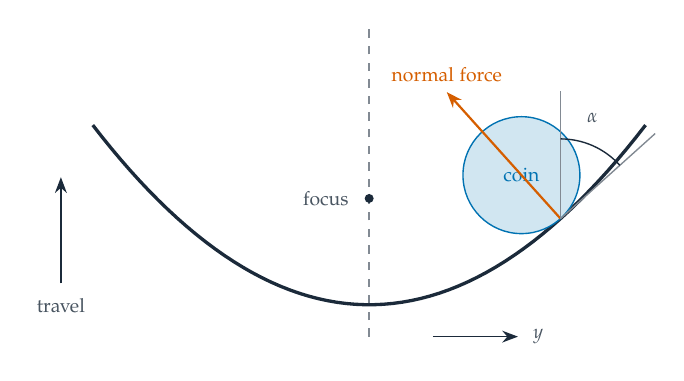
\begin{tikzpicture}[scale=1.35]
      % parabola x = y^2/(4f) with f = 1, drawn with the travel direction upward
      \draw[ink, line width=1.2pt, domain=-2.6:2.6, samples=60] plot (\x,{\x*\x/4});
      \draw[dashed, draw=ink!55] (0,-0.3) -- (0,2.6);
      \fill[ink] (0,1) circle (1.2pt);
      \node[note, anchor=east] at (-0.1,1.0) {focus};
      % contact point at y = 1.8, inward unit normal (-0.669, 0.743)
      \coordinate (P) at (1.8,0.81);
      \draw[draw=cA, fill=cA!18] ($(P)+(-0.368,0.409)$) circle (0.55);
      \node[note, text=cA] at ($(P)+(-0.368,0.409)$) {coin};
      \draw[->, cB, line width=0.8pt] (P) -- ($(P)+(-1.07,1.19)$);
      \node[note, text=cB, anchor=south] at ($(P)+(-1.07,1.19)$) {normal force};
      % tangent and the direction of travel through the contact point
      \draw[draw=ink!55] (P) -- ($(P)+(0.89,0.80)$);
      \draw[draw=ink!55] (P) -- ($(P)+(0,1.2)$);
      \draw[draw=ink] ($(P)+(0,0.75)$) arc (90:42:0.75);
      \node[note] at ($(P)+(0.3,0.95)$) {$\alpha$};
      \draw[->, line width=0.8pt] (-2.9,0.2) -- (-2.9,1.2);
      \node[note, anchor=north] at (-2.9,0.15) {travel};
      \draw[->] (0.6,-0.3) -- (1.4,-0.3);
      \node[note, anchor=west] at (1.45,-0.3) {$y$};
    \end{tikzpicture}
    \caption{A coin in contact with a parabolic jaw}
  \end{subfigure}
  \caption{The gripper. A coin touched by a jaw is pushed along the normal of the profile,
  which has an inward component everywhere except at the vertex.}
  \label{fig:gripper}
\end{figure}

The mechanics of this can be stated simply (\cref{fig:gripper}b). Let the profile be the
parabola $y^2=4fx$ with focal length $f$, opening in the direction of travel, and let the
robot advance onto a coin that lies at a lateral offset $y$ from the axis. The jaw meets the
coin with a surface inclined at an angle $\alpha$ to the direction of travel, where
\begin{equation}
  \tan\alpha = \frac{\mathrm{d}y}{\mathrm{d}x} = \frac{2f}{y}.
\end{equation}
The contact force lies within the friction angle $\varphi=\arctan\mu$ of the surface normal.
The coin slides along the jaw, towards the axis, as long as the direction of travel lies
outside that friction cone, that is, as long as $90^\circ-\alpha>\varphi$. With
$\tan\alpha=2f/y$ this gives
\begin{equation}
  \lvert y\rvert > 2\mu f .
  \label{eq:centring}
\end{equation}
A coin that meets the jaw further from the axis than $2\mu f$ is carried inward; inside
that band friction is able to hold it where it is. Two conclusions follow. The centring
improves with a short focal length and a slippery jaw, and the tips of the jaws, where
$\alpha$ is small, are where it works best, which is where a misaligned approach makes
first contact. For the friction coefficient of 0.35 used for the coin in the simulation, the
band is $0.7f$ on either side of the axis. I have not measured the focal length of the
printed jaws, and \cref{eq:centring} is given as the design rule and not as a verified
figure. When the jaws close, the coin is centred in any case, since the closed jaws leave it
little room.

\subsubsection{Release Ridges}
Each jaw carries a ridge on its inner side, near the pivot (\cref{fig:gripper}a). When the
jaws open, the ridges swing forward and push the coin out of the throat. Without them a coin
could stay against the gears as the robot backs away and be drawn back with it. With them
the coin is left where it was released. This detail decided whether a coin placed in a bin
stayed there.

\subsubsection{Actuation}
One MG995 servo drives the gripper. Its shaft turns one jaw directly, and a pair of involute
gears with equal numbers of teeth turns the other jaw by the same angle in the opposite
sense. The pivots are 25\unit{mm} apart, so each gear has a pitch diameter of 25\unit{mm}.
An involute profile keeps the velocity ratio constant through the mesh~\cite{shigley},
and equal gears make the motion of the two jaws symmetrical without any linkage.

At 4.8\unit{V} the servo is rated at 8.5\unit{kg\,cm}, which is 0.83\unit{N\,m}, and at
$60^\circ$ in 0.20\unit{s}, which is 5.2\unit{rad/s}. At the tip of a jaw, 90\unit{mm} from
the pivot, the stall torque corresponds to a force of 9\unit{N}, two orders of magnitude
above the 0.08\unit{N} needed to slide a coin. The jaws travel between an open position at
$-1.0\unit{rad}$ and a closed position at $0.09\unit{rad}$ of the driven jaw; the jaws touch
one another at about $0.096\unit{rad}$. The stroke of 1.09\unit{rad} takes 0.21\unit{s} at
the rated speed, and the mission software allows one second for it. In the pose in which the
assembly was exported, the second jaw is $7.25^\circ$ away from the mirror image of the
first, so the jaws meet slightly to one side of the centre line. This is an error of
assembly in the CAD model that the simulation reproduces.

\subsection{Sensor Placement}
\label{sec:sensors-mech}
\subsubsection{Depth Camera}
The camera looks forward from a height of 85\unit{mm}. Its depth image has a vertical field
of view of $58^\circ$, so the lowest ray leaves the lens $29^\circ$ below the horizontal and
reaches the floor at a distance
\begin{equation}
  x_{\min} = \frac{h_c}{\tan 29^\circ} = \frac{85\unit{mm}}{0.554} \approx 0.15\unit{m}
  \label{eq:blind}
\end{equation}
ahead of the lens (\cref{fig:blind}). Depth is in addition not reported below a range of
0.2\unit{m}. A caged coin lies about 4\unit{cm} ahead of the lens. The camera therefore
never sees the coin it is about to pick, nor the last 15\unit{cm} of floor in front of the
robot. This is the most important constraint that the mechanical design places on the
software, and \cref{sec:docking} describes how the infrared array takes over where the
camera ends.

\begin{figure}[htbp]
  \centering
  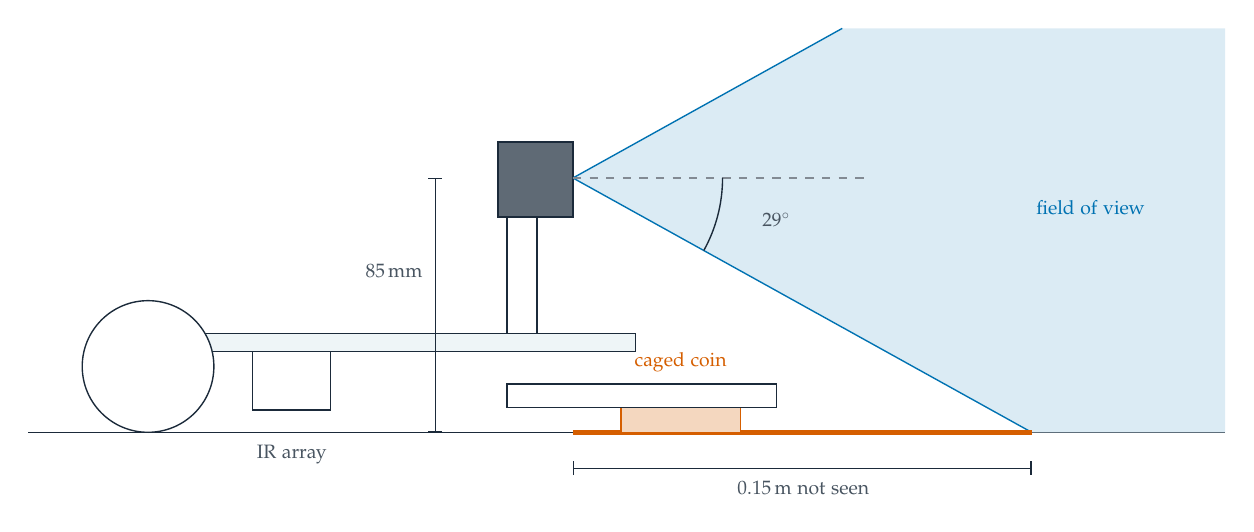
\begin{tikzpicture}[scale=0.38]
    % units: 10 mm, side view. Lens at x = 14.2, height 8.5.
    \draw[draw=ink] (-4,0) -- (36,0);
    % chassis plate and wheel
    \draw[draw=ink, fill=panel] (-1.7,2.7) rectangle (16.3,3.3);
    \draw[draw=ink, fill=white] (0,2.2) circle (2.2);
    % camera post and body
    \draw[draw=ink, fill=white] (12.0,3.3) rectangle (13.0,7.2);
    \draw[draw=ink, fill=ink!70] (11.7,7.2) rectangle (14.2,9.7);
    % field of view
    \fill[cA!14] (14.2,8.5) -- (29.53,0) -- (36,0) -- (36,13.5) -- (23.2,13.5) -- cycle;
    \draw[cA] (14.2,8.5) -- (29.53,0);
    \draw[cA] (14.2,8.5) -- (23.2,13.5);
    \draw[dashed, draw=ink!55] (14.2,8.5) -- (24,8.5);
    \draw[draw=ink] (19.2,8.5) arc (0:-29:5);
    \node[note] at (21.0,7.1) {$29^\circ$};
    % blind zone
    \draw[cB, line width=1.6pt] (14.2,0) -- (29.53,0);
    \draw[|-|] (14.2,-1.2) -- (29.53,-1.2);
    \node[note, below] at (21.9,-1.3) {0.15\,m not seen};
    % coin
    \draw[draw=cB, fill=cB!25] (15.8,0) rectangle (19.8,1.5);
    \node[note, text=cB, anchor=south] at (17.8,1.7) {caged coin};
    % jaws
    \draw[draw=ink, fill=white] (12.0,0.82) rectangle (21.0,1.62);
    % IR array
    \draw[draw=ink, fill=white] (3.5,0.74) rectangle (6.1,2.7);
    \node[note, anchor=north] at (4.8,-0.1) {IR array};
    % height
    \draw[|-|] (9.6,0) -- (9.6,8.5);
    \node[note, anchor=east] at (9.5,5.4) {85\,mm};
    \node[note, text=cA] at (31.5,7.5) {field of view};
  \end{tikzpicture}
  \caption{Side view of the front of the robot, to scale. The floor closer than 0.15\unit{m}
  to the lens is below the field of view of the depth camera, and so is a coin between the
  jaws.}
  \label{fig:blind}
\end{figure}

The holder places the camera 54\unit{mm} to the left of the centre line, beside the servo.
The offset is known to the software through the robot description, so it does not bias the
map, but it is the cause of the lateral shift of the centre of mass found in \cref{sec:mass}.

\subsubsection{Infrared Array}
The array has eight reflectance channels in a row across the robot, 15\unit{mm} apart, which
gives it a span of 105\unit{mm} between the outer channels. Its sensing face is 7.4\unit{mm}
above the floor. Two properties of its position matter later. It is 48\unit{mm} ahead of the
axle, and this distance acts as a look-ahead that damps the line follower
(\cref{sec:linefollower}). And it is 72\unit{mm} behind the gripper pivots, so that a marking
on the floor under the array fixes the position of the jaws relative to that marking; the
pick and drop markings of the arena are placed accordingly (\cref{sec:arena}).

\subsection{Manufacture}
\label{sec:manufacture}
The chassis, the jaws, the gears and the camera holder are printed in PLA. Holes and
pockets were toleranced for the bolts and nuts in use, and the chassis was printed in more
than four iterations to find clearances that the printer reproduced. All bolts have
hexagon socket heads, which take a higher tightening torque from a key than a slotted or
cross head does from a screwdriver and are standard in prototype work.

\section{Electronics and Sensing}
\label{sec:electronics}

This section is short by intent. It records what the design notes, the photographs of the
robot and the simulation model establish about the electronics, and nothing beyond that. No
circuit diagram or parts list of the competition robot was available when this report was
written.

\subsection{Actuators}
Two N20 gearmotors with encoder boards drive the wheels, and one MG995 servo drives the
gripper (\cref{sec:drive,sec:gripper}). The motors were selected for their size.

\subsection{Sensors}
\begin{description}
  \item[Infrared array.] Eight analog reflectance channels at a pitch of 15\unit{mm}, read as
        voltages between 0\unit{V} on a black surface and 5\unit{V} on a white one. The
        array serves the line following and, in the simulated mission, the final approach to
        every station.
  \item[Depth camera.] An Intel RealSense D435, which provides a colour image and a depth
        image. In the simulation it is the only sensor used for mapping, localisation,
        obstacle detection and the reading of QR codes.
  \item[Wheel encoders.] One on each motor, the source of wheel odometry.
  \item[Inertial sensor.] The simulation model carries an inertial sensor of the MPU6050
        class, flat on the plate between the wheels, whose yaw rate is fused with the wheel
        odometry (\cref{sec:odometry}).
\end{description}

\subsection{Power and Control}
The photograph of the robot (\cref{fig:v2-intro}b) shows a battery with an XT60 connector
at the rear of the plate, a step-down converter module, and a
microcontroller board on a prototyping board with a solderless breadboard for the signal
wiring. Both the electronics and the mechanical design were checked extensively before the
competition.

\subsection{The Failure at the State Round}
In the state round the infrared array stopped working and the robot could not follow the
line, so the task was not completed. The cause was not
established afterwards, and I do not speculate on it here. Two consequences are drawn for
the design. The line following depended on a single sensor with no fallback. And the photograph shows
signal wiring on a solderless breadboard, which is not a reliable connection on a moving
robot. A soldered or connectorised harness, and a check of all eight channels against known
black and white references at power-up, are the corrections proposed
in \cref{sec:discussion}.

\section{Simulation Model}
\label{sec:simulation}

The simulation runs in Gazebo Fortress with ROS~2 Humble, inside a Docker container that is
not privileged and receives only the graphics card, the display socket and the joystick
devices of the host. One script builds the image, starts the container and launches every
configuration described below.

\subsection{From CAD to a Robot Description}
\label{sec:urdf}
The CAD assembly was exported from SolidWorks as a URDF description with one mesh per link.
An export of this kind is a starting point and not a usable model. The description used
here is maintained by hand on top of the export, and it differs from it in the following
ways.
\begin{itemize}
  \item A frame \code{base\_footprint} on the floor was added below \code{base\_link}, which
        stays at the midpoint of the axle, as REP~105 prescribes~\cite{rep105}.
  \item The wheel axes were turned so that a positive rotation drives the robot forward.
  \item The right wheel was made coaxial with the left one. The export had placed it
        0.5\unit{mm} higher.
  \item The limits, effort, velocity and damping of the gripper joints, all zero in the
        export, were filled in from the data of the servo.
  \item The body of the depth camera, which was not part of the CAD assembly, was added as a
        box of $90\times25\times25\unit{mm}$ and 72\unit{g}, together with the depth and
        optical frames that the camera driver publishes.
  \item The infrared array was given a mass. The export had assigned none, and the simulator
        rejects a link without mass.
\end{itemize}

\paragraph{Collision geometry.} The visual mesh of the chassis has 277\,864 triangles. For
contact it is replaced by primitives: a box for the plate, a box for the volume above it, a
cylinder for each wheel and a sphere for the caster. The jaws and the camera holder keep
their meshes, of about 2\,000 and 700 triangles, because the shape of the jaws is what the
gripper depends on.

\paragraph{The caster.} In the CAD model the bottom of the caster dome is 0.74\unit{mm}
above the plane on which the wheels stand, so the robot would rock on it. The collision
sphere of the model is sized to touch the floor exactly. The description records this as a
correction to be made on the physical part.

\subsection{Drive and Contact}
\label{sec:sim-drive}
The wheels are driven by the differential-drive system of Gazebo, which converts a velocity
command into wheel speeds by \cref{eq:diffdrive} and publishes wheel odometry at
30\unit{Hz}. The physics step is 1\unit{ms}. The friction coefficients are 1.0 for the
wheels, 0 for the caster, 0.8 for the jaws and 0.35 for the coins.

The drive is limited to 1.0\unit{m/s^2} and 8\unit{rad/s^2}, in acceleration and in
braking. The braking limit was added after the first runs: without it the wheels stopped
at once, and the robot skidded and turned. \Cref{sec:mass}
gives the reason, a wheel load of 18\,\% of the weight, and the limit of
\cref{eq:traction} that the chosen value respects.

\subsection{Gripper}
The two jaw joints are position-controlled at the rated speed of the servo. Gazebo Fortress
ignores the mimic relation by which a URDF couples one joint to another, so the gear pair is
reproduced in software: a node receives the commanded angle of the driven jaw, clamps it to
the joint limits, rejects values that are not finite, and sends the angle to one jaw and its
negative to the other.

\subsection{Sensor Models}
\label{sec:sensor-models}
\paragraph{Depth camera.} The camera is simulated as an RGB-D sensor at the position of the
left infrared imager of the D435, with the depth field of view of the real camera,
$87^\circ\times58^\circ$, an image of $848\times480$ pixels, a depth range from 0.2 to
10\unit{m} and Gaussian image noise with a standard deviation of 0.007. The topic names
match those of the driver of the real camera, so that the same nodes can run on the
hardware. The point cloud is computed in ROS from the depth image, because the cloud that
the simulator produces is expressed in a different axis convention under the same frame
name.

\paragraph{Infrared array.} Gazebo has no reflectance sensor. Each channel is therefore
modelled by a camera of $8\times8$ pixels that looks straight down from the sensing face
and covers a spot about 8\unit{mm} across on the floor, comparable to the spot of a
reflectance sensor at that height. A node averages the brightness of each small image,
scales it to a voltage between 0 and 5\unit{V}, adds Gaussian noise, and publishes the eight
voltages at 20\unit{Hz}. A channel that lies over the edge of a line therefore returns an
intermediate voltage, as the real sensor does, and it is this that allows the position of a
line to be interpolated between channels (\cref{sec:linefollower}). The arena is lit evenly
and without shadows, so that the readings do not depend on the heading of the robot. In the
mission runs the noise has a standard deviation of 0.05\unit{V}.

\paragraph{Inertial sensor.} The inertial sensor is sampled at 100\unit{Hz}, with Gaussian
noise of 0.002\unit{rad/s} on the angular rate and 0.02\unit{m/s^2} on the acceleration.

\subsection{What the Model Leaves Out}
The motors are ideal velocity sources within the acceleration limits: there is no model of
the gear train, of backlash or of the motor driver. The servo is an ideal position source.
The encoders have no quantisation. The infrared model has no dependence on ambient light or
on the height of the array above the floor. The floor is flat. These omissions bound what
the results of \cref{sec:results} can say about the hardware, and \cref{sec:discussion}
returns to them.

\section{Arena Design}
\label{sec:arena}

The arena is a model of the task and does not reproduce the competition field. It keeps the structure of the task: a line to follow, then a
room in which coins are collected at one wall and delivered, by colour, to another. It was
designed together with the robot model, and most of its dimensions follow from two numbers
of \cref{sec:mechanical}: the pitch of the infrared array and the blind zone of the camera.

\subsection{Layout}
The field measures $3.6\times2.4\unit{m}$ and is enclosed by walls 0.3\unit{m} high
(\cref{fig:arena}). A partition with a doorway 0.8\unit{m} wide divides it into an entry
lane and a room. The robot starts in the lane on a black line, which leads through an S-bend
of two arcs of 0.6\unit{m} radius, through the doorway, to a black start square. Three pick
bays lie along the left wall and three drop zones along the front wall. Up to three boxes of
$100\times100\times150\unit{mm}$ stand in the room as obstacles.

\begin{figure}[htbp]
  \centering
  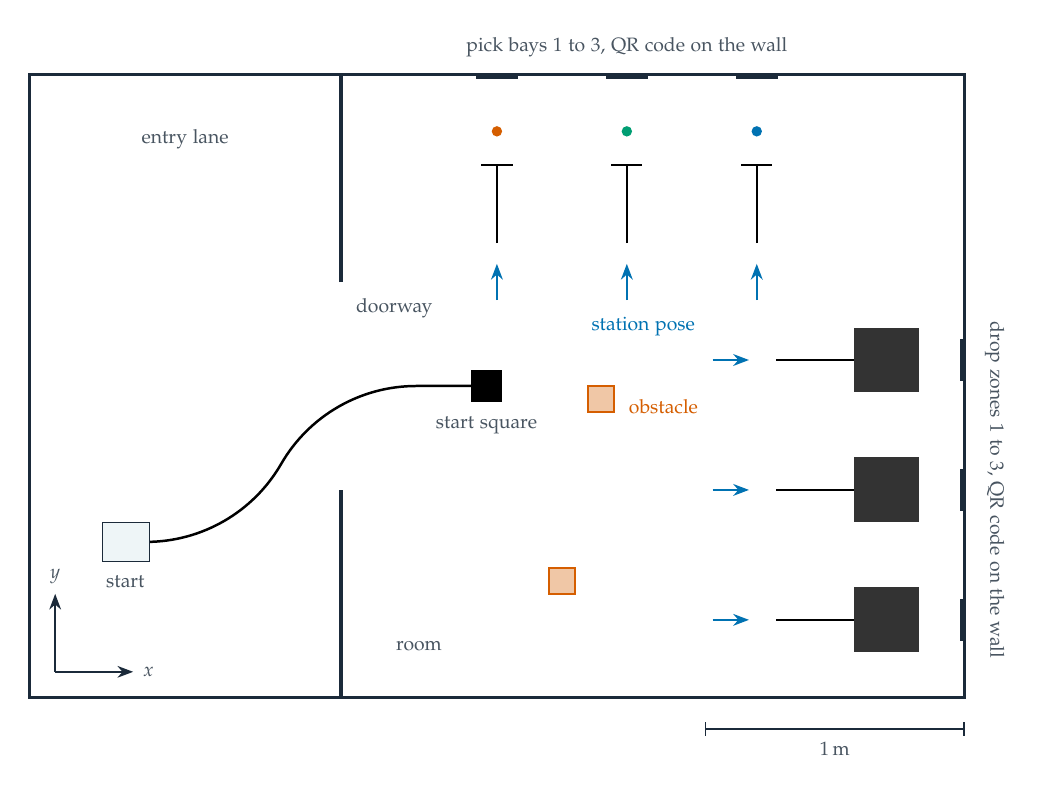
\begin{tikzpicture}[x=3.3cm, y=3.3cm]
    \arenaplan
    \arenacoins
    \arenaobstacles{1.90/0.55, 1.75/-0.15}
    % robot at the start, heading +x
    \draw[draw=ink, fill=panel] (-0.017,-0.075) rectangle (0.163,0.075);
    \node[note, anchor=north] at (0.07,-0.09) {start};
    % station poses
    \foreach \bx in {1.5,2.0,2.5} { \draw[->, cA, line width=0.8pt] (\bx,0.93) -- (\bx,1.07); }
    \foreach \dy in {0.7,0.2,-0.3} { \draw[->, cA, line width=0.8pt] (2.33,\dy) -- (2.47,\dy); }
    % labels
    \node[note] at (0.3,1.55) {entry lane};
    \node[note] at (1.2,-0.4) {room};
    \node[note, anchor=south] at (2.0,1.83) {pick bays 1 to 3, QR code on the wall};
    \node[note, rotate=-90, anchor=south] at (3.34,0.2) {drop zones 1 to 3, QR code on the wall};
    \node[note, anchor=north] at (1.46,0.52) {start square};
    \node[note, anchor=west] at (0.92,0.9) {doorway};
    \node[note, text=cB, anchor=west] at (1.97,0.52) {obstacle};
    \node[note, text=cA, anchor=east] at (2.3,0.83) {station pose};
    % axes and scale
    \draw[->] (-0.2,-0.5) -- (0.1,-0.5) node[note, right] {$x$};
    \draw[->] (-0.2,-0.5) -- (-0.2,-0.2) node[note, above] {$y$};
    \draw[|-|] (2.3,-0.72) -- (3.3,-0.72);
    \node[note, below] at (2.8,-0.73) {1\,m};
  \end{tikzpicture}
  \caption{Plan of the arena, to scale, with obstacle preset a. The arrows are the station
  poses at which the navigation hands over to the line follower.}
  \label{fig:arena}
\end{figure}

\subsection{Floor Markings Dimensioned from the Array}
\label{sec:markings}
The infrared array has eight channels at a pitch of $p=15\unit{mm}$ and a span of
105\unit{mm}. Three kinds of marking are derived from these two numbers (\cref{fig:markings}).
\begin{description}
  \item[Lines are 12\unit{mm} wide.] A line narrower than one pitch can never cover two
        channels completely. At most two neighbouring channels respond to it, each
        partially, and the ratio of their readings gives the position of the line between
        them.
  \item[Markers are 120\unit{mm} wide.] The start square and the crossbars of the pick
        bays are wider than the whole array, so that all eight channels go dark together
        when the array reaches one. Nothing else on the floor can produce that pattern, and
        a line, which darkens two channels at most, cannot be mistaken for it.
  \item[Drop squares are 250\unit{mm} wide.] The robot releases a coin when the array
        reaches the near edge of the square. The coin then lies 0.13\unit{m} further in,
        which is 5\unit{mm} from the centre of a square of this size.
\end{description}

\begin{figure}[htbp]
  \centering
  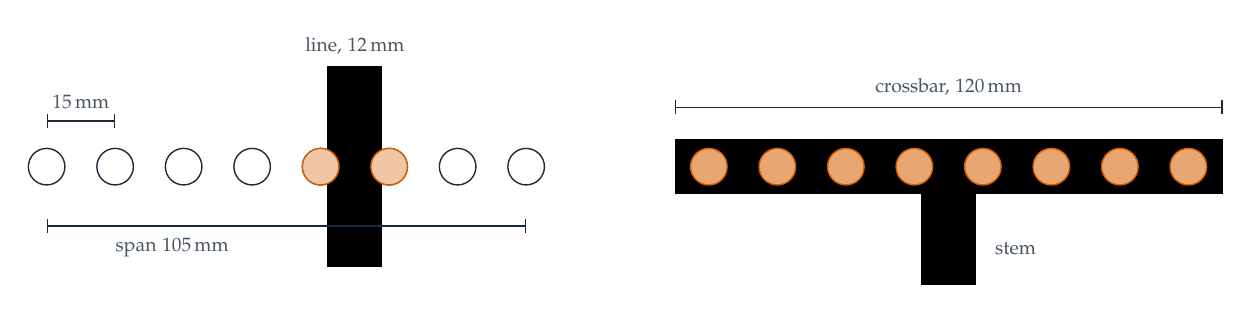
\begin{tikzpicture}[scale=0.58]
    % units: 10 mm. Left: array over a line. Right: array over a crossbar.
    \begin{scope}
      \fill[black] (0.9,-2.2) rectangle (2.1,2.2);
      \foreach \i in {0,...,7} {
        \draw[draw=ink, fill=white] ({(\i-3.5)*1.5},0) circle (0.4);
      }
      \draw[draw=cB, fill=cB!35] (0.75,0) circle (0.4);
      \draw[draw=cB, fill=cB!35] (2.25,0) circle (0.4);
      \draw[|-|] (-5.25,-1.3) -- (5.25,-1.3);
      \node[note, below] at (-2.5,-1.35) {span 105\,mm};
      \draw[|-|] (-5.25,1.0) -- (-3.75,1.0);
      \node[note, above] at (-4.5,1.05) {15\,mm};
      \node[note, above] at (1.5,2.25) {line, 12\,mm};
    \end{scope}
    \begin{scope}[xshift=14.5cm]
      \fill[black] (-6,-0.6) rectangle (6,0.6);
      \fill[black] (-0.6,-2.6) rectangle (0.6,-0.6);
      \foreach \i in {0,...,7} {
        \draw[draw=cB, fill=cB!55] ({(\i-3.5)*1.5},0) circle (0.4);
      }
      \draw[|-|] (-6,1.3) -- (6,1.3);
      \node[note, above] at (0,1.35) {crossbar, 120\,mm};
      \node[note, anchor=west] at (0.8,-1.8) {stem};
    \end{scope}
  \end{tikzpicture}
  \caption{The infrared array over a line and over a marker, to scale. The circles are the
  spots of the eight channels. A line darkens two channels at most, a marker all eight.}
  \label{fig:markings}
\end{figure}

\subsection{Stations Placed for the Blind Zone}
\label{sec:stations}
The camera does not see the last 0.15\unit{m} of floor (\cref{eq:blind}). A pick bay is
therefore a T on the floor: a stem 0.30\unit{m} long that leads to a crossbar, with the coin
0.13\unit{m} beyond the crossbar. The distance of 0.13\unit{m} is the distance from the
array to the space between the open jaws, so that a robot which stops with its array on the
crossbar has the coin between its jaws. A drop zone is a stem of the same length that ends
in the drop square.

The navigation brings the robot to a station pose on the extension of the stem and short of
its foot, 0.15\unit{m} for the bays and 0.175\unit{m} for the drop zones, and facing along
it. From there the line follower drives straight until the array finds the stem
(\cref{sec:docking}). The length of the stem is what absorbs the error of the navigation: a
lateral error of a few centimetres at the foot is steered out before the crossbar is
reached.

\subsection{QR Codes and Wall Textures}
A QR code of 160\unit{mm}, centred 0.11\unit{m} above the floor, is mounted on the wall
behind every station. It encodes the name of a colour. At a pick bay it names the colour of
the coin, and at a drop zone the colour that the zone accepts. The codes are generated with
the highest level of error correction and a wide quiet zone, so that they remain readable
when seen at an angle. The assignment of colours to bays and to zones is a launch argument,
which makes each of the 36 combinations of pick order and drop order a different mission.

Plain walls have no visual features, and a visual SLAM system cannot localise against them.
The walls therefore carry generated textures with dense, irregular detail. They exist only
for this purpose.

\subsection{One Source for the Dimensions}
The world is written as a parametrised file whose dimensions are defined once at its head.
Two other files repeat a few of them: the list of station poses read by the mission, and
the positions of the drop squares read by the referee. Both name the parameters that they
mirror. A change of the arena therefore requires edits in three places, which is a known
weakness of the present arrangement.

\section{Autonomy}
\label{sec:autonomy}

\subsection{Mission and Architecture}
The mission has four parts.
\begin{enumerate}
  \item Follow the line from the start to the start square.
  \item Visit the three drop zones and read at each the colour that it accepts.
  \item For each pick bay in turn: approach it, read the colour of its coin, cage the coin,
        carry it to the drop zone of that colour and release it.
  \item Throughout, drive around obstacle boxes that are not in the map.
\end{enumerate}

The software is a set of ROS~2 packages (\cref{fig:architecture}). Odometry, mapping,
localisation, path planning and path tracking are taken from existing open-source packages
and configured for this robot. The line follower, the docking sequences, the mission state
machine and the referee are written for it (\cref{tab:sources}). The packages for
navigation and for the mission have no knowledge that they run in a simulator: everything
that exists only in simulation, including the emulation of the infrared array and the
referee, is kept in a separate package.

\begin{table}[htbp]
  \centering
  \caption{Origin of the components of the autonomy stack.}
  \label{tab:sources}
  \small
  \begin{tabular}{@{}lll@{}}
    \toprule
    Function & Solution & Source \\
    \midrule
    Odometry & filter of wheel speed and yaw rate & \code{robot\_localization}~\cite{robotlocalization} \\
    Mapping, localisation & RGB-D graph SLAM & RTAB-Map~\cite{rtabmap} \\
    Planning and tracking & NavFn, Regulated Pure Pursuit & Nav2~\cite{nav2} \\
    QR decoding & bar code reader on the colour image & ZBar~\cite{zbar} \\
    Line following & PD steering on the line offset & this work \\
    Pick and drop sequences & infrared array and odometry & this work \\
    Mission sequencing & state machine & this work \\
    Scoring & referee on simulator ground truth & this work \\
    \bottomrule
  \end{tabular}
\end{table}

\begin{figure}[htbp]
  \centering
  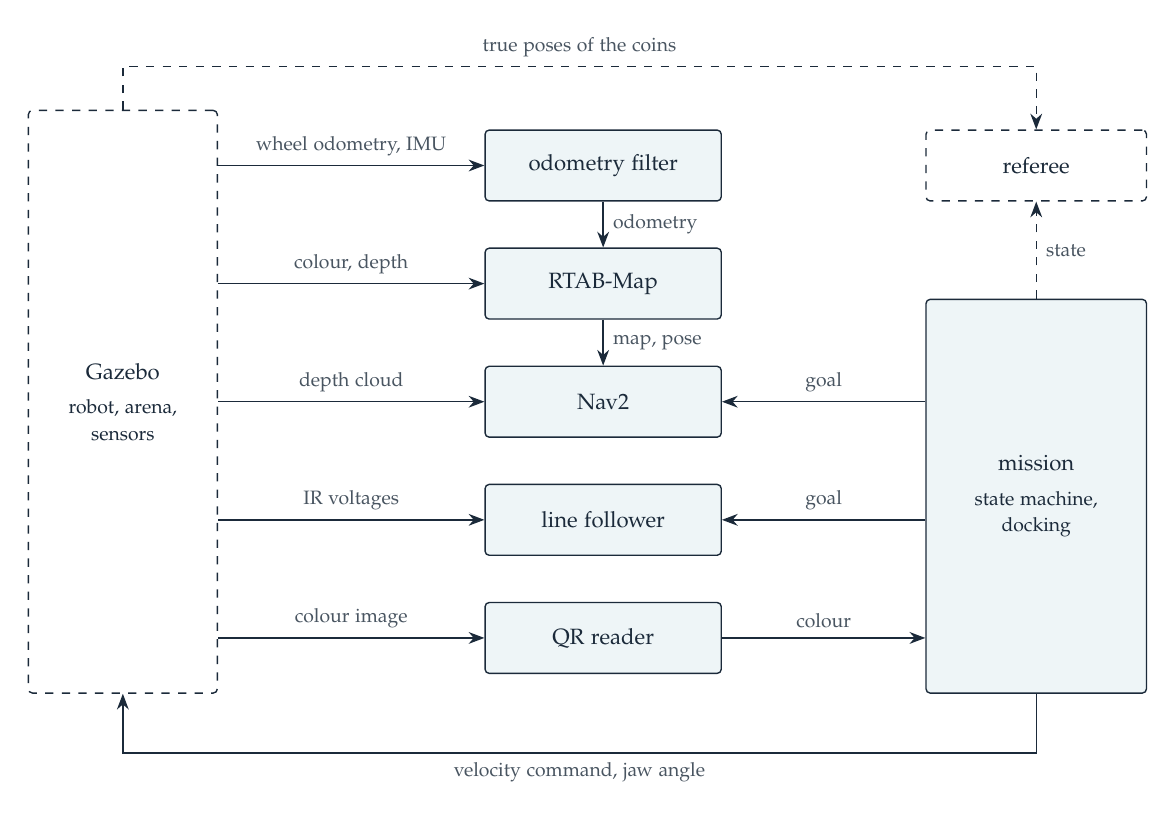
\begin{tikzpicture}
    \node[ext, minimum width=24mm, minimum height=74mm] (sim) at (0,0)
      {Gazebo\\[3pt]\scriptsize robot, arena,\\\scriptsize sensors};
    \node[box, minimum width=30mm] (ekf) at (6.1,3.0) {odometry filter};
    \node[box, minimum width=30mm] (slam) at (6.1,1.5) {RTAB-Map};
    \node[box, minimum width=30mm] (nav) at (6.1,0.0) {Nav2};
    \node[box, minimum width=30mm] (line) at (6.1,-1.5) {line follower};
    \node[box, minimum width=30mm] (qr) at (6.1,-3.0) {QR reader};
    \node[box, minimum width=28mm, minimum height=50mm] (mis) at (11.6,-1.2)
      {mission\\[3pt]\scriptsize state machine,\\\scriptsize docking};
    \node[ext, minimum width=28mm] (ref) at (11.6,3.0) {referee};
    \draw[->] (sim.east |- ekf) -- node[note, above] {wheel odometry, IMU} (ekf);
    \draw[->] (sim.east |- slam) -- node[note, above] {colour, depth} (slam);
    \draw[->] (sim.east |- nav) -- node[note, above] {depth cloud} (nav);
    \draw[->] (sim.east |- line) -- node[note, above] {IR voltages} (line);
    \draw[->] (sim.east |- qr) -- node[note, above] {colour image} (qr);
    \draw[->] (ekf) -- node[note, right] {odometry} (slam);
    \draw[->] (slam) -- node[note, right] {map, pose} (nav);
    \draw[->] (mis.west |- nav) -- node[note, above] {goal} (nav);
    \draw[->] (mis.west |- line) -- node[note, above] {goal} (line);
    \draw[->] (qr) -- node[note, above] {colour} (mis.west |- qr);
    \draw[->, dashed] (mis) -- node[note, right] {state} (ref);
    \draw[->] (mis.south) -- ++(0,-0.75) -| node[note, pos=0.25, below] {velocity command, jaw angle} (sim.south);
    \draw[->, dashed] (sim.north) -- ++(0,0.55) -| node[note, pos=0.25, above] {true poses of the coins} (ref.north);
  \end{tikzpicture}
  \caption{Software architecture. Solid boxes run unchanged on a real robot; dashed boxes
  exist only in simulation. Velocity commands are issued by Nav2, by the line follower or by
  the mission itself, one at a time, because the mission waits for each step to finish before
  it starts the next.}
  \label{fig:architecture}
\end{figure}

\subsection{Odometry}
\label{sec:odometry}
An extended Kalman filter in planar mode fuses the forward speed from the wheel encoders
with the yaw rate from the gyroscope, at 30\unit{Hz}. The yaw rate of the wheel odometry is
deliberately left out: when the robot turns on the spot the wheels slip, and the gyroscope
is the better source. The filter publishes the transform from the odometry frame to the
robot.

\subsection{Mapping and Localisation}
\label{sec:slam}
\paragraph{Building the map.} The map is built once, in the empty arena. A survey node
sends a fixed route of seven stops to the navigation and turns the robot through a full
circle at each stop, so that the camera sees every wall, while RTAB-Map adds a node to its
graph every 10\unit{cm} or 0.2\unit{rad} of travel. The route ends at the start pose and
closes the loop there. Because the survey starts at the start pose, the map frame coincides
with the frame of the arena, and the station poses can be written in arena coordinates. The
map is constrained to the plane, and its occupancy grid has cells of 2\unit{cm}. Points
below 3\unit{cm} are treated as floor, which keeps coins out of the map.

\paragraph{Localising in it.} A mission run loads the whole map and starts at its origin,
where the robot stands. Each time RTAB-Map recognises a view, twice a second at most, it
corrects the transform from the map to the odometry frame. Between corrections the pose is
carried by the odometry filter.

\paragraph{Look-alike views.} The arena contains the same QR code in two places, once at a
pick bay and once at a drop zone. Seen from close by, a code fills much of the image, and a
match of the features of the code alone was enough for RTAB-Map to conclude that the robot
stood in front of the other wall. The pose then jumped across the room. The remedy is a
condition on how the matched features are spread over the image: a view of the room matches
across the whole width of the walls, a view of a code only within the code. The walls fill a
low band of the image, and during development real views scored between 0.004 and 0.014 on
this measure and look-alikes below 0.0025; the threshold is set at 0.005. The choice is a
compromise. A threshold at the lower end of the real range rejects some true matches, and
one set higher rejects them all, after which the robot runs on odometry alone. In addition,
every new fix is checked against the last fifty views and the odometry between them.

\subsection{Navigation}
\label{sec:navigation}
Between stations the robot is driven by Nav2. The global planner is NavFn on a costmap of
2\unit{cm} cells built from the saved map, and the path is planned again once a second,
which is what steers the robot around boxes that are not in the map. The path is tracked by
the Regulated Pure Pursuit controller at 0.15\unit{m/s} with a look-ahead of 0.20\unit{m},
and the robot is turned on the spot when the path departs from its heading by more than
0.5\unit{rad}. A goal counts as reached within 2\unit{cm} and 0.05\unit{rad}.

Obstacles enter the costmaps from the depth image, reduced to every fourth pixel and to
cells of 2\unit{cm}. Points between 3\unit{cm} and 0.40\unit{m} above the floor mark
obstacles, and rays through free space clear them. The robot is treated as a disc of
0.13\unit{m} radius, and obstacles are inflated by 0.25\unit{m}.

Three properties of the robot shape the configuration.
\begin{itemize}
  \item The camera looks forward only. The controller is not allowed to reverse, and the
        recovery that backs the robot up is removed from the behaviour tree. The remaining
        recoveries clear the costmaps, turn the robot through a quarter circle to look
        around, and wait.
  \item Low objects do not reach the costmap. This is intended for coins and sensor noise,
        and it means that an obstacle lower than 3\unit{cm} would not be avoided.
  \item Turns on the spot are slow, 0.3 to 0.6\unit{rad/s}, so that successive camera views
        overlap and the localisation can follow.
\end{itemize}

\subsection{Line Follower}
\label{sec:linefollower}
\paragraph{Line position.} Each voltage $V_i$ is converted to a darkness
$d_i=1-V_i/V_{\mathrm{ref}}$ between 0 on white and 1 on black. Readings below 0.15 are set
to zero, so that noise on the white floor carries no weight. The offset of the line from the
centre of the array is the weighted mean
\begin{equation}
  e = p\,\frac{\sum_i d_i\,(i-3.5)}{\sum_i d_i}, \qquad i=0,\dots,7,
  \label{eq:offset}
\end{equation}
with $p$ the pitch. It is positive when the line is to the left. Because a line narrower
than the pitch darkens two neighbouring channels partially (\cref{sec:markings}), $e$ varies
continuously as the line moves across the array, and the resolution is much finer than the
pitch.

\paragraph{Steering.} The robot drives at a constant speed $v$ and steers with
\begin{equation}
  \omega = \operatorname{sat}_{\omega_{\max}}\bigl(k_p\,e + k_d\,\dot e\bigr),
  \label{eq:steer}
\end{equation}
with $k_p=45\unit{rad/s}$ per metre, $k_d=2\unit{rad/s}$ per metre per second and
$\omega_{\max}=1.5\unit{rad/s}$, at 20\unit{Hz}. If the line leaves the array, the robot
turns at 0.6\unit{rad/s} towards the side on which the line was last seen. If no line has
been seen yet, it drives straight, so that a goal may start a little short of a stem.

\paragraph{Why the position of the array matters.} Let the array be a distance $L$ ahead of
the axle, let $\psi$ be the heading of the robot relative to a straight line, and let $y$ be
the lateral position of the array relative to the line, so that $e=-y$. For small angles,
\begin{equation}
  \dot y = v\,\psi + L\,\omega, \qquad \dot\psi = \omega .
\end{equation}
With the proportional part of \cref{eq:steer}, $\omega=-k_p\,y$, this gives
\begin{equation}
  \ddot y + L\,k_p\,\dot y + v\,k_p\,y = 0,
  \label{eq:line-dynamics}
\end{equation}
a second-order system with natural frequency $\omega_n=\sqrt{v\,k_p}$ and damping ratio
$\zeta=\tfrac{1}{2}L\sqrt{k_p/v}$. The damping comes entirely from $L$: an array on the axle
($L=0$) would give an undamped oscillation under proportional control, whatever the gain.
With $L=48\unit{mm}$ and $k_p=45$, the damping ratio is 0.51 at the entry speed of
0.10\unit{m/s} and 0.72 at the docking speed of 0.05\unit{m/s}. The derivative term raises
the first value slightly, to 0.53. The mechanical decision to hang the array ahead of the
axle is thus what makes a simple controller sufficient, and driving the stems slowly is what
makes the approach to a marker well damped.

\paragraph{Markers.} A marker is reported when at least six channels have a darkness of 0.5
or more in two successive samples. A line darkens two channels at most, so only a square or
a crossbar can do this, and the requirement of two samples rejects a single noisy reading.
Two sample periods at 20\unit{Hz} are 5\unit{mm} of travel at the docking speed.

The follower is offered as an action. A goal names a maximum distance and a speed, and the
result states whether a marker was reached and how far the robot drove.

\subsection{Docking}
\label{sec:docking}
A station is approached in two stages (\cref{fig:docking}). Nav2 brings the robot to the
station pose. The line follower then drives straight until the array finds the stem, steers
onto it, and stops at the marker. Everything after that is a timed movement of the jaws or
a straight move measured by odometry.

\begin{description}
  \item[Pick.] Open the jaws. Follow the stem to the crossbar, at which point the coin is
        between the jaws. Read the QR code on the wall. Close the jaws. Back out by the
        distance just driven.
  \item[Drop.] Follow the stem until the array enters the square. Open the jaws, which
        pushes the coin clear. Back out, then close the jaws.
  \item[Read.] Follow the stem to its marker, read the QR code and back out. This is used
        for the survey of the drop zones.
\end{description}
The robot backs out along the stem that it has just driven and by the distance that it
measured, which is the only reverse movement in the mission. It needs no sensing behind the
robot because the path has just been traversed.

\begin{figure}[htbp]
  \centering
  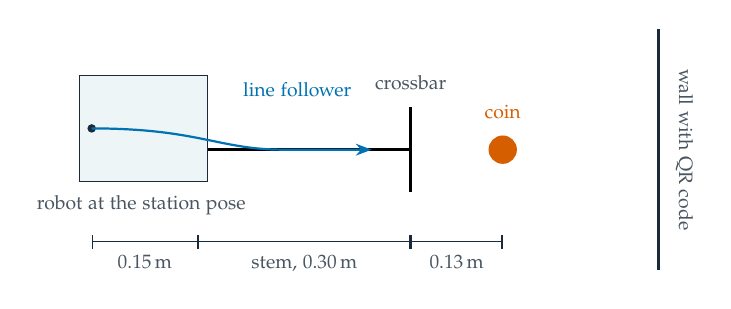
\begin{tikzpicture}[x=9cm, y=9cm]
    % pick bay drawn with the approach direction to the right (x along the stem)
    \draw[draw=ink, line width=1.1pt] (0.95,-0.17) -- (0.95,0.17);
    \node[note, rotate=-90, anchor=south] at (0.96,0) {wall with QR code};
    \draw[draw=black, line width=1.2pt] (0.30,0) -- (0.60,0);
    \draw[draw=black, line width=1.2pt] (0.60,-0.06) -- (0.60,0.06);
    \fill[cB] (0.73,0) circle (0.02);
    \node[note, anchor=south, text=cB] at (0.73,0.03) {coin};
    % station pose with a lateral error
    \draw[draw=ink, fill=panel] (0.133,-0.045) rectangle (0.313,0.105);
    \fill[ink] (0.15,0.03) circle (0.006);
    \draw[->, cA, line width=0.8pt] (0.15,0.03) .. controls (0.30,0.03) and (0.33,0.0) .. (0.42,0.0) -- (0.545,0.0);
    \node[note, anchor=north] at (0.22,-0.05) {robot at the station pose};
    \node[note, anchor=south, text=cA] at (0.44,0.06) {line follower};
    \draw[|-|] (0.15,-0.13) -- (0.30,-0.13);
    \node[note, below] at (0.225,-0.135) {0.15\,m};
    \draw[|-|] (0.30,-0.13) -- (0.60,-0.13);
    \node[note, below] at (0.45,-0.135) {stem, 0.30\,m};
    \draw[|-|] (0.60,-0.13) -- (0.73,-0.13);
    \node[note, below] at (0.665,-0.135) {0.13\,m};
    \node[note, anchor=south] at (0.60,0.07) {crossbar};
  \end{tikzpicture}
  \caption{Approach to a pick bay, to scale. The navigation leaves the robot at the station
  pose with an error of a few centimetres; the line follower removes it along the stem and
  stops the array on the crossbar, with the coin between the open jaws.}
  \label{fig:docking}
\end{figure}

\paragraph{QR codes are read at the station only.} The decoder reports the text of a code
but not where the code is in the image. A code is therefore trusted only when the robot
stands at the marker in front of it, where no neighbouring code is in view, and only after
three identical decodes in a row. Decodes received before the robot arrived are discarded,
so that a code passed on the way is never taken for the code of the station.

\subsection{Mission State Machine}
\label{sec:statemachine}
The mission is a sequence of blocking steps, and the state machine only decides what happens
next (\cref{fig:states}). Its failure handling is deliberately plain.
\begin{itemize}
  \item If the start square is not found within 3\unit{m} of travel, the mission fails.
  \item If a marker is not found at a station, the robot backs out and tries the station once
        more.
  \item A drop zone whose code cannot be read is left out of the table of colours.
  \item A coin whose code cannot be read is left in its bay, with the jaws still open, since
        without a colour there is nowhere to take it.
  \item A coin whose colour has no known drop zone is set down where the robot stands.
\end{itemize}
The mission reports success only when all three coins have been delivered.

\begin{figure}[htbp]
  \centering
  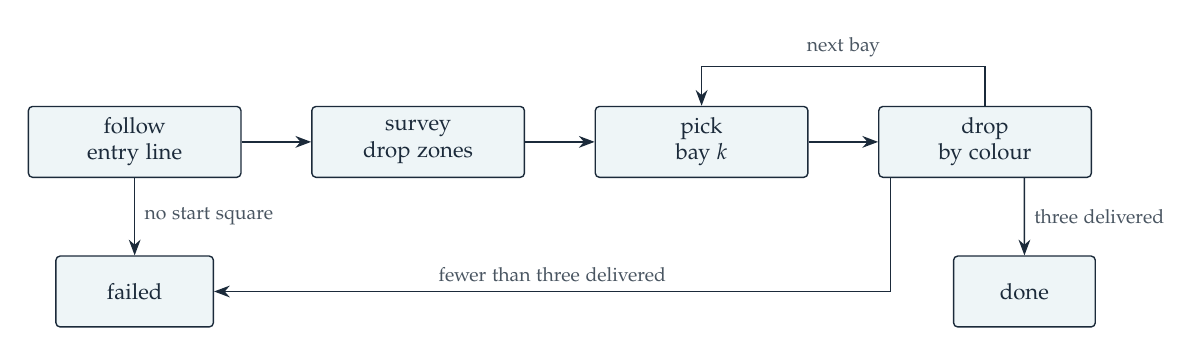
\begin{tikzpicture}
    \node[box, minimum width=27mm] (a) at (0,0) {follow\\entry line};
    \node[box, minimum width=27mm] (b) at (3.6,0) {survey\\drop zones};
    \node[box, minimum width=27mm] (c) at (7.2,0) {pick\\bay $k$};
    \node[box, minimum width=27mm] (d) at (10.8,0) {drop\\by colour};
    \node[box, minimum width=18mm] (e) at (11.3,-1.9) {done};
    \node[box, minimum width=20mm] (f) at (0,-1.9) {failed};
    \draw[->] (a) -- (b); \draw[->] (b) -- (c); \draw[->] (c) -- (d);
    \draw[->] (d.north) -- ++(0,0.5) -| node[note, pos=0.25, above] {next bay} (c.north);
    \draw[->] ([xshift=5mm]d.south) -- node[note, right] {three delivered} (e.north);
    \draw[->] (a) -- node[note, right] {no start square} (f);
    \draw[->] ([xshift=-12mm]d.south) |- node[note, pos=0.75, above] {fewer than three delivered} (f.east);
  \end{tikzpicture}
  \caption{States of the mission.}
  \label{fig:states}
\end{figure}

\subsection{Referee}
\label{sec:referee}
A run is scored by a referee that reads the true positions of the coins from the simulator.
A coin is home when its centre lies inside the drop square whose QR code names its colour.
The referee has no connection to the robot other than the state of the mission, which tells
it when to give its verdict, and nothing on the robot may read the ground truth. A run
passes when all three coins are home at the end.

\section{Results}
\label{sec:results}
% Figures of the results section, drawn from the files in docs/latex/data.

\newcommand{\figpath}{%
\begin{figure}[htbp]
  \centering
  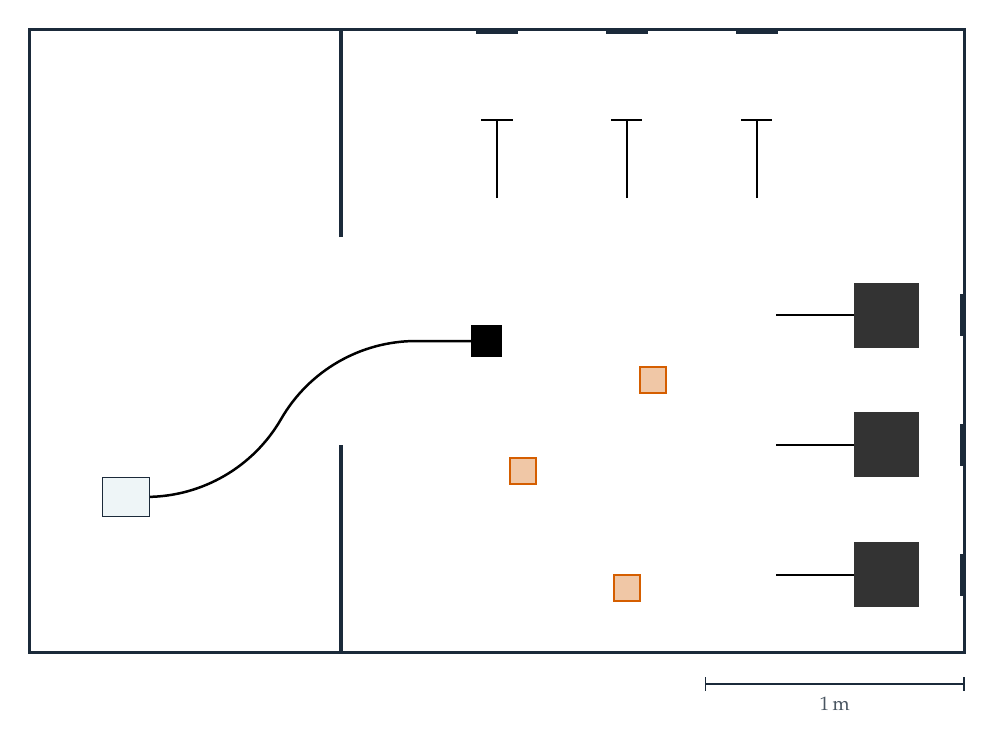
\begin{tikzpicture}[x=3.3cm, y=3.3cm]
    \arenaplan
    \arenaobstacles{2.10/0.45, 1.60/0.10, 2.00/-0.35}
    \draw[cA, line width=0.5pt, line join=round] plot file {../data/track_m03.dat};
    \draw[draw=ink, fill=panel] (-0.017,-0.075) rectangle (0.163,0.075);
    \draw[|-|] (2.3,-0.72) -- (3.3,-0.72);
    \node[note, below] at (2.8,-0.73) {1\,m};
  \end{tikzpicture}
  \caption{True path of the robot in run 3 (obstacle preset b, three boxes). The path
  follows the entry line, visits the three drop zones, and then alternates between the pick
  bays and the drop zones, passing the boxes on whichever side the planner finds free.}
  \label{fig:path}
\end{figure}}

\newcommand{\figtimes}{%
\begin{figure}[htbp]
  \centering
  \begin{tikzpicture}
    \begin{axis}[report, ybar stacked, bar width=9pt, ymin=0, ymax=340,
        xlabel={run}, ylabel={simulated time [s]}, xtick={1,...,12}, enlarge x limits=0.06,
        area legend, grid=none, ymajorgrids]
      \addplot[fill=cD!55, draw=cD] table[x expr=\coordindex+1, y=t_line, col sep=comma] {../data/runs.csv};
      \addplot[fill=cA, draw=cA] table[x expr=\coordindex+1, y=t_survey, col sep=comma] {../data/runs.csv};
      \addplot[fill=cB!70, draw=cB] table[x expr=\coordindex+1, y=t_coins, col sep=comma] {../data/runs.csv};
      \legend{entry line, survey of drop zones, three coins}
    \end{axis}
  \end{tikzpicture}
  \caption{Duration of the three parts of the mission in each run.}
  \label{fig:times}
\end{figure}}

\newcommand{\figslam}{%
\begin{figure}[htbp]
  \centering
  \begin{tikzpicture}
    \begin{axis}[report, xlabel={simulated time [s]}, ylabel={position error [mm]},
        xmin=0, xmax=310, ymin=0, ymax=45, legend columns=-1]
      \addplot[cA, line width=0.6pt] table[x=t, y=err_mm] {../data/slam_m03.dat};
      \addplot[cB, line width=0.6pt] table[x=t, y=odom_mm] {../data/slam_m03.dat};
      \legend{map pose, odometry alone}
    \end{axis}
  \end{tikzpicture}
  \caption{Distance between the estimated and the true position of the robot in run 3, for
  the pose in the map and for the odometry filter alone.}
  \label{fig:slam}
\end{figure}}

\newcommand{\figdock}{%
\begin{figure}[htbp]
  \centering
  \begin{subfigure}[b]{0.48\linewidth}
    \centering
    \begin{tikzpicture}
      \begin{axis}[report, width=\linewidth, height=0.9\linewidth,
          xlabel={across the stem [mm]}, ylabel={along the stem [mm]},
          xmin=-10, xmax=10, ymin=-10, ymax=10, axis equal image]
        \fill[black!25] (axis cs:-10,-6) rectangle (axis cs:10,6);
        \addplot[only marks, mark=*, mark size=1.3pt, cA]
          table[x=lateral_mm, y=along_mm, col sep=comma] {../data/picks.csv};
      \end{axis}
    \end{tikzpicture}
    \caption{Array centre when the jaws close}
  \end{subfigure}\hfill
  \begin{subfigure}[b]{0.48\linewidth}
    \centering
    \begin{tikzpicture}
      \begin{axis}[report, width=\linewidth, height=0.9\linewidth,
          xlabel={along the stem [mm]}, ylabel={across the stem [mm]},
          xmin=-25, xmax=25, ymin=-25, ymax=25, axis equal image]
        \addplot[only marks, mark=*, mark size=1.3pt, cB]
          table[x=dx_mm, y=dy_mm, col sep=comma] {../data/drops.csv};
      \end{axis}
    \end{tikzpicture}
    \caption{Coin after release}
  \end{subfigure}
  \caption{Docking accuracy over all picks and drops. (a) Position of the centre of the
  infrared array relative to the centre of the crossbar at the moment the jaws close; the
  grey band is the crossbar, 12\unit{mm} wide. (b) Final position of each coin relative to
  the centre of its drop square, which extends to $\pm125\unit{mm}$.}
  \label{fig:dock}
\end{figure}}

\newcommand{\figline}{%
\begin{figure}[htbp]
  \centering
  \begin{tikzpicture}
    \begin{axis}[report, width=0.8\linewidth, height=0.36\linewidth,
        xlabel={distance along the arena, $x$ [m]}, ylabel={offset from the line [mm]},
        xmin=0, xmax=1.45, ymin=-12, ymax=12, legend columns=-1]
      \addplot[cD, line width=0.6pt] table[x=x, y=err_mm] {../data/line_n0.0_v0.10.dat};
      \addplot[cA, line width=0.6pt] table[x=x, y=err_mm] {../data/line_n0.05_v0.10.dat};
      \addplot[cB, line width=0.6pt] table[x=x, y=err_mm] {../data/line_n1.0_v0.10.dat};
      \legend{no noise, 0.05\,V, 1.0\,V}
    \end{axis}
  \end{tikzpicture}
  \caption{Offset of the array centre from the entry line at 0.10\unit{m/s}, for three
  levels of noise on the infrared readings. The two arcs of the S-bend lie between
  $x=0.15$ and $1.19\unit{m}$.}
  \label{fig:line}
\end{figure}}


All results in this section were obtained in the simulation of \cref{sec:simulation}, in
the arena of \cref{sec:arena}, with the parameters of \cref{app:parameters}. Times are
simulated time. Positions called true are the ground truth of the simulator.

\subsection{Method}
The mission was run twelve times without a display: three runs for each of the four
obstacle layouts (none and the presets a, b and c), with a different combination of pick
order and drop order in almost every run (\cref{tab:runs}). All runs used the same map,
built once in the empty arena, and the same start pose. The noise on the infrared readings
was 0.05\unit{V}. Each run was recorded as described in \cref{sec:verification} and scored
by the referee.

\subsection{Outcome of the Mission}
All twelve runs passed: in every run the referee found all three coins inside the drop
squares of their colours, 36 coins of 36. No station needed a second attempt, no QR code
was missed, and the navigation entered no recovery behaviour in any run.

\begin{table}[htbp]
  \centering
  \caption{The twelve mission runs. Pick and drop give the colours of bays 1 to 3 and of
  drop zones 1 to 3. Map error is the RMS distance between the pose in the map and the true
  pose; line error is the RMS offset of the array from the entry line.}
  \label{tab:runs}
  \begin{tabular}{@{}cccccccc@{}}
    \toprule
    Run & Pick & Drop & Obstacles & Coins home & Time [s] & Path [m] & Map error [mm] \\
    \midrule
    1 & RGB & BRG & a & 3 of 3 & 301 & 18.4 & 8.4 \\
    2 & RGB & BRG & none & 3 of 3 & 300 & 18.0 & 8.8 \\
    3 & GBR & RGB & b & 3 of 3 & 307 & 18.7 & 10.7 \\
    4 & BRG & GRB & c & 3 of 3 & 305 & 17.9 & 10.6 \\
    5 & RBG & RGB & none & 3 of 3 & 299 & 17.7 & 11.8 \\
    6 & GRB & BGR & a & 3 of 3 & 299 & 18.4 & 11.8 \\
    7 & BGR & RBG & b & 3 of 3 & 304 & 18.6 & 9.2 \\
    8 & RGB & GBR & c & 3 of 3 & 292 & 17.6 & 10.0 \\
    9 & GBR & BRG & none & 3 of 3 & 298 & 17.5 & 9.7 \\
    10 & BRG & RGB & a & 3 of 3 & 295 & 17.8 & 9.8 \\
    11 & RBG & GRB & b & 3 of 3 & 300 & 18.5 & 9.7 \\
    12 & GRB & RBG & c & 3 of 3 & 298 & 17.6 & 8.2 \\
    \bottomrule
  \end{tabular}
\end{table}

A mission takes 300\unit{s} on average, between 293 and 307\unit{s} (\cref{fig:times}): 19\unit{s}
on the entry line, 83\unit{s} for the survey of the three drop zones and 198\unit{s} for the
three coins, or 66\unit{s} per coin. The robot covers 18.1\unit{m}, which is an average of
0.06\unit{m/s}; most of the time goes into turning on the spot, the slow approach along the
stems and the waiting for the jaws and for the QR codes. The obstacles cost little. The
mean time is 299\unit{s} without obstacles and 304\unit{s} with the three boxes of
preset b, and the paths differ by less than a metre. \Cref{fig:path} shows the true path of
one run.

\figpath
\figtimes

\subsection{Line Following}
\label{sec:res-line}
On the entry line of the twelve missions, the centre of the array stayed within 6.0\unit{mm}
of the centre of the line, with an RMS offset of 1.6\unit{mm} (1.4 to 2.1\unit{mm} over the
runs). The line is 12\unit{mm} wide and the channels are 15\unit{mm} apart, so the offset is
a tenth of the pitch: the interpolation between partially covered channels
(\cref{eq:offset}) works as intended. In every run the array stopped on the start square.

The line follower was also run on its own on the entry line, once for each of several noise
levels and speeds (\cref{tab:line,fig:line}). Two results stand out. The follower is
insensitive to noise up to 0.2\unit{V}, four times the level used in the missions, because
readings below the floor threshold carry no weight. At 0.5\unit{V} noise crosses that
threshold and the offset grows fourfold, and at 1.0\unit{V} it reaches 46\unit{mm}, close
to the half span of the array, although the line was not lost. And the offset grows quickly
with speed: 1.1\unit{mm} at the docking speed, 1.7\unit{mm} at the entry speed, and
17.6\unit{mm} at 0.30\unit{m/s}. This agrees in direction with \cref{eq:line-dynamics},
where the damping ratio falls with the square root of the speed, from 0.72 at
0.05\unit{m/s} to 0.29 at 0.30\unit{m/s}. The speeds chosen for the mission are on the
well-damped side.

\begin{table}[htbp]
  \centering
  \caption{Line follower alone on the entry line, one run per row. Offset of the array
  centre from the centre of the line.}
  \label{tab:line}
  \begin{tabular}{@{}ccccc@{}}
    \toprule
    Noise [V] & Speed [m/s] & RMS offset [mm] & Largest offset [mm] & Start square reached \\
    \midrule
    0 & 0.10 & 1.5 & 4.0 & yes \\
    0.05 & 0.10 & 1.7 & 4.3 & yes \\
    0.2 & 0.10 & 1.9 & 4.1 & yes \\
    0.5 & 0.10 & 6.8 & 19.7 & yes \\
    1.0 & 0.10 & 18.0 & 45.9 & yes \\
    \midrule
    0.05 & 0.05 & 1.1 & 2.8 & yes \\
    0.05 & 0.15 & 3.3 & 7.7 & yes \\
    0.05 & 0.20 & 7.4 & 16.3 & yes \\
    0.05 & 0.30 & 17.6 & 37.9 & yes \\
    \bottomrule
  \end{tabular}
\end{table}

\figline

\subsection{Localisation}
\label{sec:res-slam}
Over the part of each mission that is driven in the room, the pose in the map differed
from the true pose by 9.9\unit{mm} RMS (8.2 to 11.8\unit{mm} over the runs). The 95th
percentile was 19\unit{mm} on average, the largest error in any run 39\unit{mm}, and the
heading error 0.7\unit{^\circ} RMS. These errors are below the goal tolerance of the
navigation, 20\unit{mm}, for most of the time, and well below the lateral error that a stem
can absorb.

This result has to be read with a second one (\cref{fig:slam}). The odometry filter alone,
without any correction from the map, was never more than 30\unit{mm} from the truth in any
run, and ended a mission of 18\unit{m} with an error of 16\unit{mm} on average. In this
simulation the odometry is nearly ideal: the encoders have no quantisation, the floor is
uniform and the drive stays inside its traction limit. The map therefore has little to
correct, and its corrections are of the same size as the error they remove. The runs show
that the localisation is stable over five minutes and does not jump, which was the failure
described in \cref{sec:slam}; they do not show how much it would contribute on a real
floor, where wheel odometry drifts.

\figslam

\subsection{Docking}
\label{sec:res-dock}
\Cref{fig:dock} gives the accuracy of the two movements on which the manipulation depends,
over all 36 picks and 36 drops.

\paragraph{Pick.} At the moment the jaws closed, the centre of the array was 2.7\unit{mm}
RMS to the side of the stem, with a largest offset of 7.1\unit{mm}, and on average
2.9\unit{mm} past the centre of the crossbar (0.9 to 6.0\unit{mm}), that is, always on the
bar. The heading differed from the direction of the stem by 2.9\unit{^\circ} RMS and by
7.1\unit{^\circ} at most. The heading is the least well controlled quantity: a stem of
0.30\unit{m} removes a lateral error faster than it removes the turn that the correction
itself introduces. All 36 coins were nevertheless caged, which is the tolerance that the
shape of the jaws was designed to provide.

\paragraph{Drop.} The coins came to rest 9.0\unit{mm} from the centres of their squares on
average and 20.7\unit{mm} at most. The square extends 125\unit{mm} from its centre, so the
margin is a factor of six. The offsets are not centred: every coin lies between 5 and
11\unit{mm} short of the centre along the stem, which is the distance by which the coin
sits further back between the jaws than the nominal 0.13\unit{m}.

\figdock

\subsection{The Simulated Robot}
\Cref{fig:sim-shots} shows the simulation during a mission.

\begin{figure}[htbp]
  \centering
  \begin{subfigure}[b]{0.49\linewidth}
    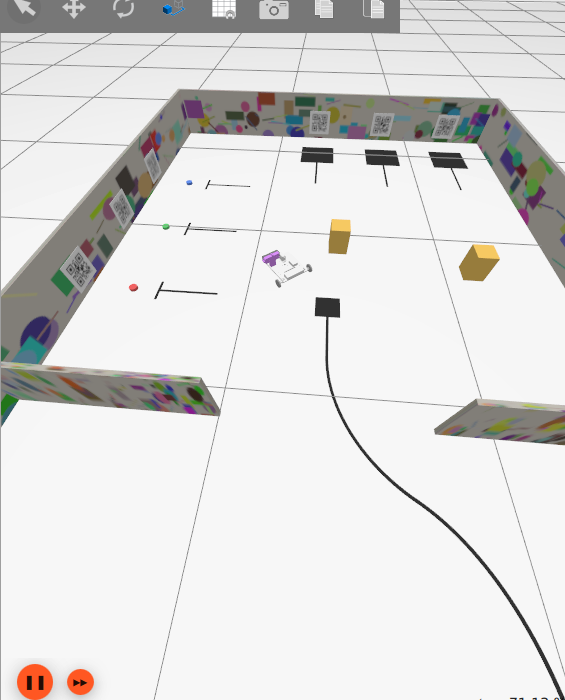
\includegraphics[width=\linewidth]{sim_arena.png}
    \caption{Entry line and room in Gazebo}
  \end{subfigure}\hfill
  \begin{subfigure}[b]{0.49\linewidth}
    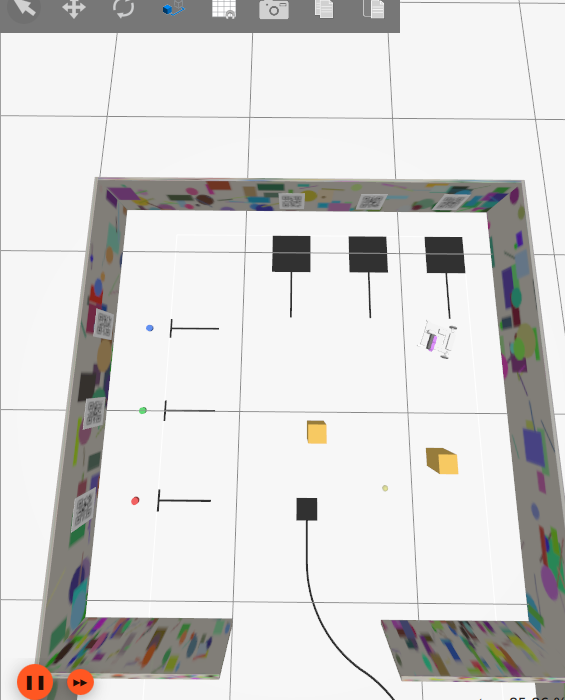
\includegraphics[width=\linewidth]{sim_pick.png}
    \caption{Robot in the room, seen from above the entry lane}
  \end{subfigure}\\[4pt]
  \begin{subfigure}[b]{0.8\linewidth}
    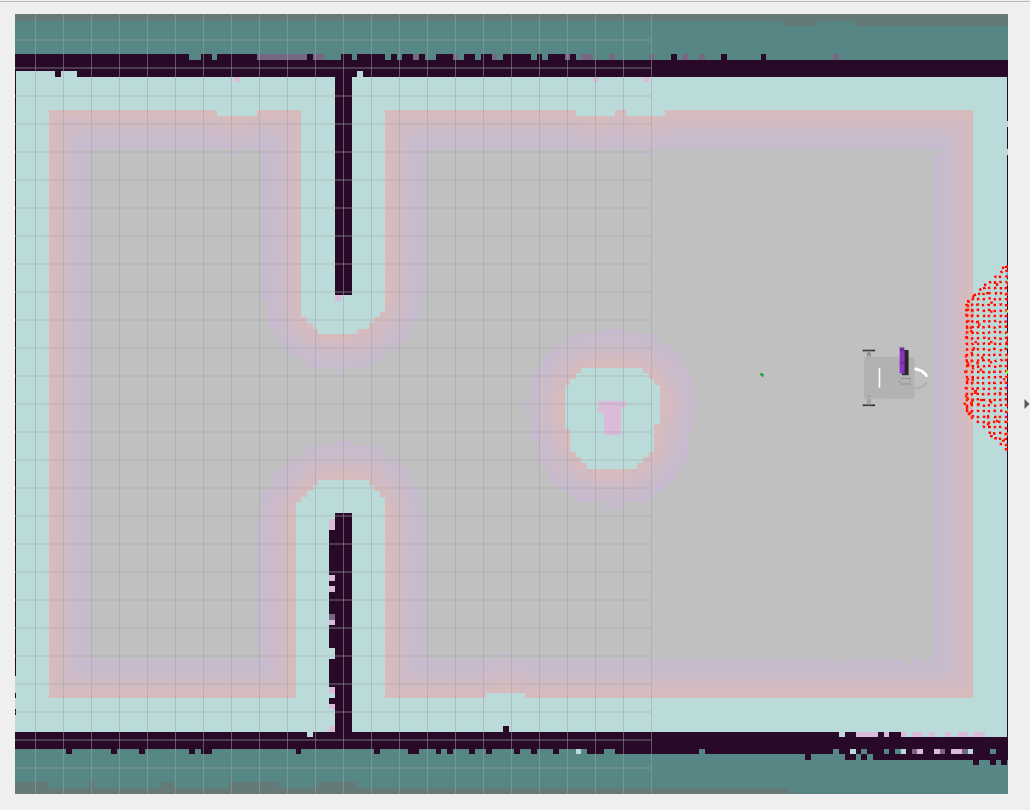
\includegraphics[width=\linewidth]{sim_rviz.png}
    \caption{Map and inflated costmap in RViz, with the robot at a drop zone}
  \end{subfigure}
  \caption{The simulated mission.}
  \label{fig:sim-shots}
\end{figure}

\subsection{Summary}
\begin{itemize}
  \item The mission succeeded in twelve of twelve runs, with four obstacle layouts and
        eleven combinations of colours, in 300\unit{s} on average.
  \item The line follower holds the line within 6\unit{mm} at the speeds used, tolerates
        four times the nominal sensor noise, and degrades with speed as the analysis of its
        damping predicts.
  \item The pose in the map is accurate to 10\unit{mm} RMS, but the simulated odometry is
        nearly as good, so the simulation does not test the value of the map.
  \item The robot stops on a crossbar within 7\unit{mm} laterally and places coins within
        21\unit{mm} of the centre of a square of 250\unit{mm}.
\end{itemize}

\section{Verification}
\label{sec:verification}

\subsection{Unit Tests}
The arithmetic of the mission is kept in two modules that do not import ROS~2: the line
mathematics (offset, marker detection and steering) and the table of stations and colours.
They are covered by 13 unit tests, which run in under a second without the simulator. The
tests fix the behaviour that the rest of the mission relies on:
\begin{itemize}
  \item a floor without a line gives no offset, and a line between the middle channels gives
        an offset of zero;
  \item a line under the leftmost channel gives a positive offset and one under the
        rightmost a negative offset, which fixes the sign convention against the channel
        order of the robot description;
  \item readings below the floor threshold are ignored;
  \item a marker requires its number of dark channels in successive samples, and a single
        sample of a line in between resets the count;
  \item the steering turns towards the line, saturates at its limit, and its derivative
        term opposes an error that is closing;
  \item the station file holds three bays and three drop zones, the table matches colours
        to zones, and an unknown colour is rejected.
\end{itemize}
All 13 tests pass on the code as measured in \cref{sec:results}.

\subsection{Scoring Against Ground Truth}
A mission can report success and still have failed, for example when a coin slips out of
the jaws on the way and the robot releases nothing. The verdict on a run is therefore not
taken from the mission but from the referee of \cref{sec:referee}, which reads the true
positions of the coins. The two are separated in the software as well: the ground truth is
bridged from the simulator on a topic of its own, and no node of the robot subscribes to it.

\subsection{Recording}
The measurements of \cref{sec:results} were taken by a recording node that only listens. It
logs, at 10\unit{Hz} of simulated time, the true pose of the robot, the pose estimated by
the localisation and the pose of the odometry, together with every change of mission state,
every command to the jaws and every line of the referee. The scripts that run the missions
and evaluate the recordings are kept with the report, so that every number in it can be
reproduced.

\section{Discussion and Limitations}
\label{sec:discussion}

\subsection{Validity of the Results}
Four limitations apply to the results of \cref{sec:results} and determine how far they may
be generalised.

\paragraph{Simulation only.} Every measurement in this report was taken in the simulation.
None was taken on the printed robot, for which there is no recorded data beyond the
photographs and the outcome of the two competition rounds. The simulated motors are ideal
within their limits, the floor is flat and evenly lit, and the infrared model has no
dependence on ambient light. The results show that the software is correct with respect to
its own model; they do not predict the performance of the hardware.

\paragraph{A model built on CAD values.} The mass properties on which \cref{sec:mass} rests
are those that the CAD program calculated. The robot was not weighed, and the motor data in
the model are placeholders. The conclusions drawn there are large enough to survive
moderate errors, since a wheel load of 18\,\% would have to be wrong by a factor of several
before the conclusion changed, but the figures are not measurements.

\paragraph{A favourable arena.} The arena was designed together with the software. Its
markings have the widths that the array needs, its walls have the textures that the SLAM
system needs, and its lighting casts no shadows. A competition field offers none of these
by arrangement. The arena shows that the approach works when its assumptions hold, and
\cref{sec:arena} states what those assumptions are.

\paragraph{A small number of runs.} The mission was run twelve times and each line-following
condition once. The runs differ in the order of the colours and in the obstacles, not in
the start pose, the map or the lighting, and the map was the same in all of them.
Differences of a few millimetres or a few seconds between conditions are within what a
repetition could change.

\subsection{Known Issues}
\label{sec:issues}
\begin{description}
  \item[The wheels are lightly loaded.] The model puts 82\,\% of the weight on the caster
        (\cref{sec:mass}). The simulation works within the resulting traction limit only
        because the drive is limited to 1.0\unit{m/s^2}. On the hardware, the caster should
        be moved towards the gripper and the camera to the centre line, after the robot has
        been weighed on its three supports.
  \item[The caster does not reach the floor in CAD.] The dome ends 0.74\unit{mm} above the
        wheel contact plane (\cref{sec:urdf}). The simulation corrects this in its collision
        geometry; the physical part needs the same correction.
  \item[The jaws do not meet on the centre line.] The second jaw is $7.25^\circ$ off the
        mirror image of the first in the exported assembly (\cref{sec:gripper}).
  \item[The footprint used for planning is a disc.] The navigation treats the robot as a
        disc of 0.13\unit{m} radius about the midpoint of the axle. The closed jaws reach
        0.21\unit{m} ahead of that point and lie outside the disc. The inflation of the
        costmap by 0.25\unit{m} covers the difference in the present arena; a polygonal
        footprint would be the correct description.
  \item[Low obstacles are not seen.] Anything lower than 3\unit{cm} is treated as floor, and
        nothing closer than 0.15\unit{m} in front of the robot is seen at all.
  \item[Localisation depends on a threshold.] The condition that rejects look-alike views
        (\cref{sec:slam}) is a single number chosen for this arena and this camera height.
        It rejects some true matches, and a different arena would need it chosen again.
  \item[Dimensions are repeated in three files.] The station poses and the drop squares
        mirror the arena file by hand (\cref{sec:arena}).
  \item[No feedback from the jaws.] The mission assumes that a coin is caged when the array
        is on the crossbar and the jaws have had time to close. It cannot tell that a coin
        was missed or lost on the way. Only the referee sees this.
  \item[One line sensor, no fallback.] This is the failure of the state round
        (\cref{sec:electronics}), and the simulated mission has the same dependency: every
        approach ends on the infrared array.
\end{description}

\subsection{What I Would Do Differently}
Three changes follow from this work, in order of value.
\begin{enumerate}
  \item \emph{Check the mass properties during the design, not after it.} The calculation of
        \cref{sec:mass} takes minutes once the CAD model exists. Done during the fifteen
        days, it would have moved the caster and the camera before the first print.
  \item \emph{Treat the line sensor as a part that can fail.} A check of all eight channels
        on a black and a white reference at power-up, a soldered harness, and a degraded
        mode that crosses the line section on odometry and vision are the measures
        that address a failure of this kind.
  \item \emph{Build the simulation first.} The simulation was written after the competition.
        Written before it, it would have allowed the mission software to be developed
        while the parts were printing.
\end{enumerate}

\subsection{Future Work}
\begin{itemize}
  \item Weigh the printed robot on its supports, measure the motors, and replace the
        placeholder values of the model.
  \item Move the caster and the camera as proposed and repeat the analysis of \cref{sec:mass}.
  \item Run the mission on the hardware, beginning with the line follower and the docking,
        which need only the infrared array and the encoders.
  \item Add a contact or current signal from the gripper so that a missed coin is detected.
  \item Derive the station poses and the referee squares from the arena file.
  \item Vary the start pose, the lighting and the floor friction in the simulation, and
        repeat each condition several times.
\end{itemize}

\section{Conclusion}
\label{sec:conclusion}

Trident is a small robot designed around one task, and the design decisions that matter
most are the ones that removed something. The gripper has no lift axis and no sensor: two
curved jaws on a pair of equal gears cage a coin and slide it, and ridges on the jaws leave
it behind on release. The camera cannot see the floor in front of the robot, and no second
camera was added: the infrared array that follows the line also guides the last part of
every approach, and the floor markings are dimensioned from its pitch so that it can.

Two lessons recur. The first is that a model answers questions that were settled by eye
during the build. The centre of mass lies inside the support triangle, as intended, but the mass
properties of the CAD model put 82\,\% of the weight on the caster, and this, and not the
motors, limits the acceleration of the robot. The simulation showed the
consequence as a skid before the calculation explained it. The second is that the position
of a sensor is a control parameter. The damping of the line follower is set by the distance
of the array ahead of the axle, and an array on the axle would have needed a different
controller.

The simulated mission is complete: the robot follows the line, maps and localises with its
camera, drives around unmapped obstacles, and delivers the three coins by colour, scored by
a referee that it cannot see. The steps that remain are on the hardware: to weigh the robot
on its supports and move the caster and the camera accordingly, to replace the breadboard
wiring of the infrared array, and to run the mission on the printed robot.


\bibliographystyle{unsrtnat}
\bibliography{references}

\clearpage
\begin{appendices}
\section{Parameters}
\label{app:parameters}
\Cref{tab:params-sim,tab:params-mission} list the parameters of the simulation model and of
the mission as used for the measurements of \cref{sec:results}.

\begin{table}[htbp]
  \centering
  \caption{Parameters of the simulation model.}
  \label{tab:params-sim}
  \begin{tabular}{@{}ll@{}}
    \toprule
    Parameter & Value \\
    \midrule
    Physics step & 1\unit{ms} \\
    Friction: wheels, caster, jaws, coin & 1.0, 0, 0.8, 0.35 \\
    Drive limits & 1.0\unit{m/s^2}, 8.0\unit{rad/s^2} \\
    Wheel joint limits (placeholders) & 0.05\unit{N\,m}, 31.4\unit{rad/s} \\
    Jaw joint: range, effort, speed & $-1.0$ to $0.09\unit{rad}$, 0.83\unit{N\,m}, 5.2\unit{rad/s} \\
    Wheel odometry rate & 30\unit{Hz} \\
    Depth camera: image, rate & $848\times480$, 60\unit{Hz} \\
    Depth camera: field of view, range & $87^\circ\times58^\circ$, 0.2 to 10\unit{m} \\
    Infrared array: channels, rate, noise & 8, 20\unit{Hz}, 0.05\unit{V} \\
    Inertial sensor: rate, gyroscope noise & 100\unit{Hz}, 0.002\unit{rad/s} \\
    Coin: diameter, height, mass & 40\unit{mm}, 15\unit{mm}, 23.4\unit{g} \\
    \bottomrule
  \end{tabular}
\end{table}

\begin{table}[htbp]
  \centering
  \caption{Parameters of the mission and of the navigation.}
  \label{tab:params-mission}
  \begin{tabular}{@{}ll@{}}
    \toprule
    Parameter & Value \\
    \midrule
    Line follower: $k_p$, $k_d$, $\omega_{\max}$ & 45, 2, 1.5\unit{rad/s} \\
    Line follower: floor threshold, dark level & 0.15, 0.5 \\
    Marker: channels, samples & 6, 2 \\
    Speed on the entry line, on a stem & 0.10\unit{m/s}, 0.05\unit{m/s} \\
    Reach on the entry line, on a stem & 3.0\unit{m}, 0.60\unit{m} \\
    Attempts per station & 2 \\
    QR code: identical decodes, time allowed & 3, 4\unit{s} \\
    Time allowed for the jaws & 1\unit{s} \\
    Navigation speed, look-ahead & 0.15\unit{m/s}, 0.20\unit{m} \\
    Goal tolerance & 2\unit{cm}, 0.05\unit{rad} \\
    Costmap cell, robot radius, inflation & 2\unit{cm}, 0.13\unit{m}, 0.25\unit{m} \\
    Obstacle height band & 0.03 to 0.40\unit{m} \\
    Replanning rate & 1\unit{Hz} \\
    Map: node spacing, loop detection rate & 0.10\unit{m} or 0.2\unit{rad}, 2\unit{Hz} \\
    Minimum inliers, minimum inlier spread & 25, 0.005 \\
    \bottomrule
  \end{tabular}
\end{table}

\section{Running the Simulation}
\label{app:running}
All commands are given to one script on the host. The image has to be built once.
\begin{verbatim}
./docker/run.sh image      build the Docker image
./docker/run.sh up         start the container
./docker/run.sh build      build the workspace
./docker/run.sh test       unit tests of the mission logic
./docker/run.sh map        survey the empty arena and save the map
./docker/run.sh mission    run the mission with the referee
./docker/run.sh mission pick_order:=GBR drop_order:=RGB obstacles:=b
\end{verbatim}
\sloppy The measurements of \cref{sec:results} were produced by scripts kept in the folder
\code{docs/latex/figures/src}. The script \code{run\_missions.sh} runs a list of missions
without a display and records each, \code{run\_line\_sweep.sh} does the same for the line
follower alone, and \code{analyse\_runs.py} and \code{analyse\_line.py} evaluate the
recordings.

\end{appendices}

\end{document}
